% !TeX spellcheck = <none>
\documentclass[UTF8]{ctexart}

\CTEXsetup[format={\Large\bfseries}]{section}
\usepackage{amsmath, amsfonts, amsthm, bm, enumerate, ulem}
\usepackage{epstopdf, graphicx}
\usepackage{algorithm}
\usepackage{algorithmicx}
\usepackage{algpseudocode}
\usepackage{booktabs}
\usepackage{mathrsfs}
\usepackage{geometry}
\usepackage{multirow}
\geometry{scale = 0.8}
\usepackage[colorlinks, linkcolor=red, anchorcolor = blue, citecolor=green]{hyperref}

\floatname{algorithm}{算法}
\renewcommand{\algorithmicrequire}{\textbf{输入:}}
\renewcommand{\algorithmicensure}{\textbf{输出:}}
\usepackage{listings}
\usepackage{xcolor}
\lstset{
	numbers=left,
	numberstyle= \tiny,
	keywordstyle= \color{ blue!70},
	commentstyle= \color{red!50!green!50!blue!50},
	frame=shadowbox, % 阴影效果
	rulesepcolor= \color{ red!20!green!20!blue!20} ,
	escapeinside=``, % 英文分号中可写入中文
	xleftmargin=2em,xrightmargin=2em, aboveskip=1em,
	framexleftmargin=2em
}

\theoremstyle{plain}
\newtheorem{thm}{定理}[section]
\newtheorem{lem}[thm]{引理}
\newtheorem{prop}[thm]{命题}
\newtheorem*{cor}{推论}

\theoremstyle{definition}
\newtheorem{defn}{定义}[section]
\newtheorem{conj}{猜想}[section]
\newtheorem{exmp}{例子}[section]

\theoremstyle{remark}
\newtheorem*{rem}{结论}
\newtheorem*{note}{注解}

\DeclareMathOperator*{\argmax}{argmax}
\DeclareMathOperator*{\argmin}{argmin}

\begin{document}
	\setcounter{footnote}{1}
	\title{基于跳过程与统计学习的普适排行榜类产品度量模型}
	\author{程晨\footnote{School of Mathematical Sciences, Peking University, Beijing 100871, China. Email address:
			\href{mailto:moriartycc@pku.edu.cn}{moriartycc@pku.edu.cn}, ID: 1500010714}, \quad 陈子恒\footnote{School of Mathematical Sciences, Peking University, Beijing 100871, China. }, \quad 郝天泽\footnote{School of Mathematical Sciences, Peking University, Beijing 100871, China. Email address:\href{mailto:1500010606@pku.edu.cn}{1500010606@pku.edu.cn}, ID: 1500010606}}
	\date{}
	\maketitle
	\abstract{
		
		\textbf{关键字:}
	}
	\newpage
	\tableofcontents
	\newpage
	\section{引言}
    随着互联网的快速发展,人们在日常生活中接触到的信息量大大增加。在为用户生活带来便利的同时,也很容易使得用户“迷失”在大量的信息中。为了使人们能够更加快速的获得他们所需要的信息,各类互联网公司使用了不同的方式来对信息进行筛选、分析和排序,以便于提升用户体验。例如如谷歌、百度等搜索引擎按照条目与关键词相关性、条目的点击行为发生次数、条目的浏览频次以及一些其他因素来对搜索结果进行排序;如美团、饿了吗等外卖类应用会对商家按照人气、服务、评价及特定用户光顾次数进行排序;如豆瓣等则会按照作品的热度、评分等进行排序。这样的排序以带来更大的用户价值为目的,针对不同公司相应的产品特点,采用不同的排序算法,对大量的信息进行了排序,生成了相关信息排行榜。

    一个自然的问题是:这样的排行榜是否实现了其提升用户体验的目的,又或者在多大程度上实现了其创造用户价值的目的。或者说,如何比较不同排行榜、排行算法之间优劣。为了解决这一问题,我们先考虑可以通过技术手段获得的数据以及不同的排行算法如何应用这些数据这一问题。

    通过文献调研\cite{agichtein2006improving}\cite{barrett2009enhanced}\cite{nematzadeh2017algorithmic}\cite{nie2005object}\cite{zehlike2017fa},我们发现大多数的排行算法使用了以用户点击次数、用户浏览时间、用户关于条目的反馈、用户重复点击条目的频率为代表的用户交互特征数据或是由其进一步推断出的条目对于用户的相关程度。同时,虽然已经有许多关于不同的排行算法、以及排行算法的优化相关的工作,但是就排行算法或是利用排行算法得出的排行榜本身进行评价、打分的工作比较少有。

    我们接下来的工作,就是通过可以得到的用户在不同条目上停留时间及相关决策来推断并量化出用户关于这样的排行榜的体验,这样的量化结果可以体现出这一排行榜的作用效果也可以用以比较不同排行榜产品之间的优劣,给出了一种排行榜类产品的度量模型。在对排行榜类产品进行度量时,我们将产品的实现方式视为黑箱,即无需关注其所采用的具体交互设计、技术实现、推荐算法,仅通过可获取的用户行为便可实现这一度量。

    在第二部分中,我们将就模型的基本假设进行描述。第三部分中,我们将先对一种相对简单的无跳过的顺序选择模型进行论述并提出度量模型。第四部分中,进而对带跳过的顺序选择模型进行论述并提出度量。第五部分中,对另一种带跳过的投票模型进行论述并提出度量。最终在第七部分中比较两种实际的排行榜产品(Hacker News ranking algorithm以及Reddit ranking algorithms)的表现,并基于我们上面的度量在第八部分中提出一种优化的排行榜算法。最终得到一种排行榜产品表现的量化评价方式以及优化的排行榜算法。

	\section{假设}
	在开始阐述我们的模型之前,我们先描述这些模型所依赖的一些基本假设,和所建立的概率模型的空间。
	\paragraph{排行榜} 我们所讨论的排行榜为产品状态集合$\mathcal{P}=\left\{1,2,\cdots,N \right\}$的一个排序,我们将所有排行榜产品构成的集合记为$\Omega_P$,则$\forall \omega \in \Omega_P$,我们就有一个排行榜
	$$
	\omega = (p_1,p_2,\cdots,p_N)
	$$
	\paragraph{产品固有性质} 为了能够度量排行榜类产品的“优劣”,我们假设产品本身有一些固有性质。如果直接定义一个“好坏”的程度,既难以描述和精确定义,又不适合在现实中使用。因此,我们考虑一些能够准确观察到和用统计方法推断的性质,且所有数据都能够用\textbf{用户停留时间}$\tau$和\textbf{用户决策}$a$来确定。对于任意一个产品$i \in \mathcal{P}$,我们假设
	\begin{itemize}
		\item \textbf{用户停留时间$\tau$的分布}。用户停留时间服从一个仅与$i$有关的分布$f_i$,或
		$$
		\tau \sim f_i
		$$
		我们说明这样的假设是合理的。尽管对于每一个不同的用户$u$,其所对应的$f_i^u$可能不同(我们认为一个确定的用户使用同一份产品所用的时间也是一个随机变量)。但考虑所有用户集合$\mathcal{U}$,以及每一个用户$u \in \mathcal{U}$被抽样的概率$p_u$,我们就能得到
		$$
		f_i = \sum_{u \in \mathcal{U}} f_i^u p_u
		$$
		\item \textbf{用户的决策$a$的可能性}。对于排行榜类产品,用户本身可能有多种感官或心理上的体验,但这些体验并不能被开发者观察和收集到,因此并不是我们所关心的。我们关心的是用户所做的决策,而这些决策将被用来衡量排行榜类产品的好坏。具体来说,根据我们研究的不同排行榜类模型,我们将用户的决策分为
		\begin{itemize}
			\item \textbf{接受(Accepted)}:对于选择型的排行榜,接受表示用户阅读该产品后选择了该产品。
			\item \textbf{放弃(Rejected)}:对于选择型的排行榜,放弃表示用户阅读该产品后放弃了该产品。
			\item \textbf{跳过(Skipped)}:对于选择、投票型的排行榜,跳过表示用户没有阅读该产品就直接跳过。
			\item \textbf{结束(Terminated)}:对于投票型的排行榜,结束表示用户结束了他的阅读过程。
			\item \textbf{投票(Voted)}:对于投票型的排行榜,投票表示用户阅读该产品后进行的决策,具体来说可以有三种
			\begin{itemize}
				\item \textbf{支持(Up vote)}
				\item \textbf{反对(Down vote)}
				\item \textbf{不表态(No vote)}
			\end{itemize}
		\end{itemize}
	\end{itemize}
	\paragraph{用户} 对于用户来说,我们关心他们的停留时间$\tau$和决策$a$。相应的,我们做出这些假设
	\begin{itemize}
		\item $\tau$为指数分布。即$f_i = \mathrm{Exp}(\lambda_i)$。这样的假设是常用且合理的。
		\item 用户群体对于接受、放弃、跳过、结束、支持、反对和不表态分别有基于产品的固有概率$a_i,r_i,s_i,t_i,u_i,d_i,n_i$。
		\item 产品独立性。每个用户使用当前产品时不会受到之前产品的影响,且不考虑个人喜好的因素,即其所做决策的概率完全有产品本身决定。
	\end{itemize}
	
	\section{无跳过的顺序选择模型——Steam探索队列}
	\subsection{模型概述 \& 符号约定}
	我们首先考虑一种最为简单,受约束较多的排行榜类推荐模型——\textbf{无跳过的顺序选择模型}。\textbf{在这个模型中,每一个用户必须依照排行榜的顺序依次阅读有关每一个产品的信息,不能跳过,且必须作出一个选择(我们假设如果到了排行榜队列底端就必须选择最后一个产品)}。这样的模型是基于著名的游戏品台Steam中的探索队列(\ref{modelA_fig_1})功能简化得到的。
	\begin{figure}[h!]
		\centering
		
\includegraphics[width = 12cm]{modelA_fig_1.png}
		\caption{Steam探索队列}\label{modelA_fig_1}
	\end{figure}
	Steam探索队列是Steam游戏平台为用户推荐产品的一种方式。该队列通过分析用户的喜好设定、浏览记录以及购买记录等信息为用户推荐一个产品队列(可视为一种产品排行榜)。当用户浏览此队列时,需要依次浏览队列中每一个产品的相关信息并进行是否感兴趣的选择(即接受或放弃的用户决策)。当我们假定现在客户有购买一个产品的需求,其浏览Steam探索队列的方式及可抽象为这里的无跳过的顺序选择模型。而往往这样的队列足够长,且是通过分析用户喜好得来,所以不妨假设用户可以从这一队列中挑选出一个其接受的产品,即前面谈到的如果到了排行榜队列底端就必须选择最后一个产品的假设。 \\
	
	具体来说,我们给出无跳过的顺序选择模型的定义。
	\begin{defn}\textbf{(无跳过的顺序选择模型)}该模型是一个建立在状态空间为$\mathcal{P} \cup \left\{A\right\}$上的跳过程。其中$A$表示接受状态。其中状态$i$处的指数闹钟参数为$\lambda_i$,且其嵌入链的转移概率为
	\begin{equation}
	\begin{aligned}
	a_{p_N} & = 1 \\
	\bm{P}_{p_i,A}  & = a_{p_i}  \\
	\bm{P}_{p_i,p_{i+1}} & = r_{p_i} = 1 - a_{p_i}
	\end{aligned}
	\end{equation}
	相应地,该跳过程的速率矩阵可以描述为
	\begin{equation}
	\begin{aligned}
	\bm{Q}_{p_i,A} & = \lambda_{p_i} a_{p_i} \\
	\bm{Q}_{p_i,p_{i+1}} & = \lambda_{p_i} r_{p_i} = \lambda_{p_i} ( 1 - a_{p_i})
	\end{aligned}
	\end{equation}
	在图($\ref{modelA_fig_2}$)中展示了具体的模型。该模型可表述为$\mathfrak{A}\left(\bm{\lambda}, \bm{a}, \omega\right)$。
	\end{defn}
	\begin{figure}[h!]
		\centering
		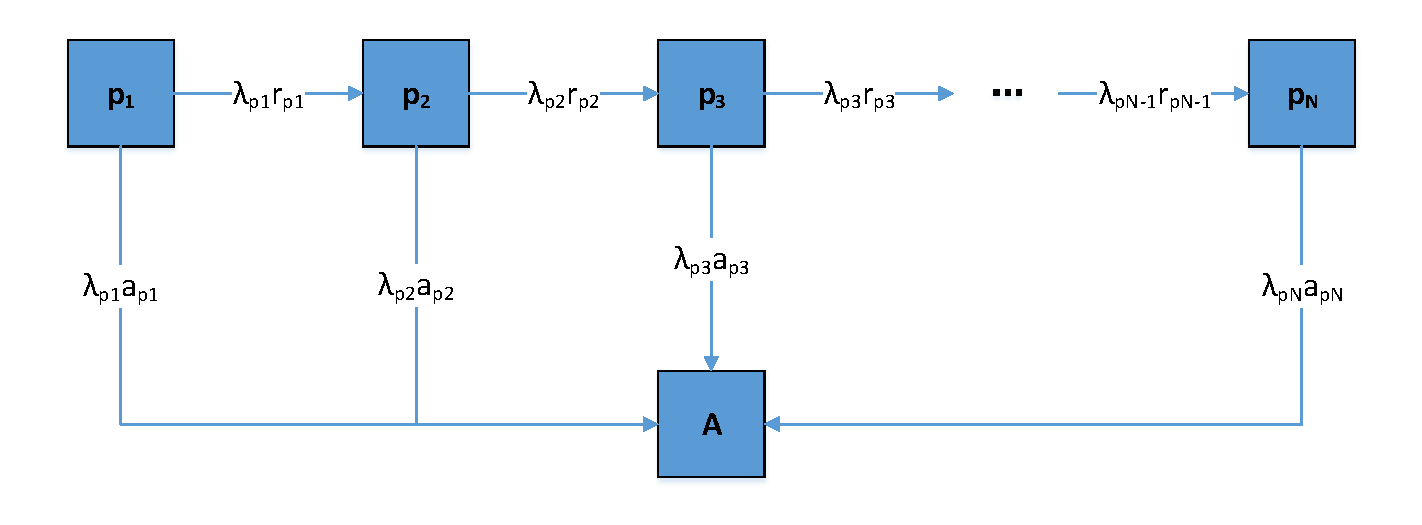
\includegraphics[width = 12cm]{modelA_fig_2.pdf}
		\caption{无跳过的顺序选择模型结构}\label{modelA_fig_2}
	\end{figure}
	直观上看,此模型实际上就是我们上面文字描述的严格定义。$A$表示接受状态,即用户决定接受某一产品,$a_{p_i}$表示决定接受产品$p_i$的概率,$r_{p_i} = 1 - a_{p_i}$表示拒绝产品$p_i$从而继续浏览$p_{i+1}$的概率,于是$\lambda_{p_i} a_{p_i}$即表示决定接受产品$p_i$的速率,$\lambda_{p_i} r_{p_i} = \lambda_{p_i} (1 - a_{p_i})$即表示拒绝产品$p_i$从而继续浏览$p_{i+1}$的速率。从而构建出了此跳过程的转移速率矩阵。
	\subsection{度量模型}
	在这样的模型中,我们有理由设置用户找到其接受的产品的时间$\tau_E$为衡量产品优劣的标准。时间越短,那么产品就越有效。而$\tau_E$在对应的随机过程中即为到达状态$E$的首达时,其分布函数可以表示为
	$$
	F_{\tau_E}(t) = e_{p_1}^T \exp(\bm{Q}t)e_{E}, \quad e_i \in \mathbb{R}^{N \times 1}, i \in \mathcal{P}
	$$
	其方差和期望分别为(约定$a_{p_0} = 1$)
	\begin{equation} \label{EQ_A}
	\begin{aligned}
	\mathbb{E} \tau_E & = \sum_{k=1}^N \frac{\prod\limits_{j=0}^{k-1}(1-a_{p_j})}{\lambda_{p_i}} \\
	\mathrm{Var} \tau_E & = \sum_{k=1}^N \left(\frac{\prod\limits_{j=0}^{k-1}(1-a_{p_j})}{\lambda_{p_i}}\right)^2
	\end{aligned}
	\end{equation}
	证明请参见附录。为了综合考虑期望和方差,以及展现出用户对于长队列的不满程度,我们将衡量函数定义为
	\begin{equation}
	\mathrm{Score}_{\mathfrak{A}\left(\bm{\lambda}, \bm{a}, \omega\right)}(x, \alpha) =  \sum_{k=1}^N \left(\frac{\prod\limits_{j=0}^{k-1}(1-a_{p_j})}{\lambda_{p_i}} x^k\right)^\alpha, \quad x \in [1, \infty), \alpha \in [1,2]
	\end{equation}
	
	其中的$x \in [1, \infty)$可以理解为某种“不满值”,即随着浏览队列的加长,用户的耐心渐渐减少,每浏览队列中越靠后的一个商品用户增加的不满值越大,因而其属于$[1, \infty)$。$\alpha \in [1,2]$则是综合考虑用户所需时间的期望与方差。对于一个优秀的排行方式,其应该尽量使得用户平均等待时间较少,所积累不满较少的同时保证用户“一致地”满意。于是我们得到了这里的衡量函数$\mathrm{Score}_{\mathfrak{A}\left(\bm{\lambda}, \bm{a}, \omega\right)}(x, \alpha)$。注意到$\alpha = 1, x = 1$时衡量函数就等于等待时间的期望,而$\alpha = 2, x = 1$时衡量函数就等于等待时间的方差,而这里“不满值”$x$也可以理解成一种“心理时间”,即在较长时间的等待后,对用户而言等待时间似乎被加长,这说明了衡量函数的合理性。 \\
	
	当然,由于参数$\bm{\lambda}, \bm{a}$是隐含的,我们需要通过统计推断的方法得到它们,即通过数据得到推断的参数$\bm{\hat{\lambda}}, \bm{\hat{a}}$,然后得到我们的衡量函数
	$$
	\mathrm{Score}_{\mathfrak{A}\left(\bm{\hat{\lambda}}, \bm{\hat{a}}, \omega\right)}(x, \alpha)
	$$
	且$\mathrm{Score}_{\mathfrak{A}\left(\bm{\hat{\lambda}}, \bm{\hat{a}}, \omega\right)}(x, \alpha)$越小,则排行榜产品越好。
	\subsection{统计推断 \& 优化算法}
	对于参数$\bm{\lambda}, \bm{a}$的推断我们使用极大似然估计,即假设第$m$个用户接受了第$p_{k_m}$个产品,前$k_m$个产品的浏览时间分别为$t_{m,i}, 1 \leq i \leq m$,总共有$M$个用户数据被收集,那么似然函数为
	\begin{equation}
	\mathcal{L}\left(\bm{\lambda}, \bm{a}, \omega\right) = \sum_{m=1}^M \ln p_k(\bm{\lambda}, \bm{a}) = \sum_{m=1}^M \ln \left(\left(\prod_{i=1}^{k_m-1}(1-a_{p_i})\right)a_{p_{k_m}}\left(\prod_{i=1}^{k_m} \lambda_{p_i}\right)\exp\left(-\sum_{i=1}^{k_m}\lambda_i t_{m,i}\right)\right)
	\end{equation}
	容易看出此对数似然函数为凸函数,我们使用成熟的凸优化工具(CVX toolbox)可以得到极大似然估计
	$$
	\left(\bm{\hat{\lambda}}, \bm{\hat{a}}\right) = \argmin_{\left(\bm{\lambda}, \bm{a}\right)} \mathcal{L}\left(\bm{\lambda}, \bm{a}, \omega\right)
	$$
	利用推断得到的参数就可以计算衡量函数了。
	\subsection{实验结果}
	为了展示模型的预测性,我们设定了两组参数,并用它们生成相应的数据和排行榜进行评分。
	
	\begin{table}[h!]
		\tiny
		\centering
		\label{tab:steam-param}
		\begin{tabular}{cc|cccccccccc|c}
			\hline
			&                                         & 1 & 2 & 3 & 4 & 5 & 6 & 7 & 8 & 9 & 10 & $\epsilon_{\text{rel}}$\\
			\hline
			\multirow{4}{*}{Set 1 \textbf{Random}}
			& $\lambda$       & 0.5050   & 0.4131  &  0.3867 &   0.6170  &  0.4310 & 0.7324 &   0.4094  &  0.3305 &   0.3052  &  0.3287 & \multirow{2}{*}{1.2512e-02} \\
		   	& $\hat{\lambda}$ & 0.4953 &   0.4139  &  0.3811  &  0.6134 &   0.4356  &  0.7327 &   0.4113   & 0.3293 &   0.2944   & 0.3214  & \\
		   	& $a$             &  0.7444  &  0.9558  &  0.9955  &  0.8685 &   0.9752 &0.7918 &   0.9294  &  0.8240  &  0.8206& $\slash$ & \multirow{2}{*}{3.7643e-03} \\
			& $\hat{a}$       &  0.7397   & 0.9559  &  0.9952  &  0.8688  &  0.9764 & 0.7928   & 0.9318 &   0.8322   & 0.8215& $\slash$ & \\
			\hline
			\multirow{4}{*}{Set 2 \textbf{Decrease}} 	& $\lambda$       & 0.5000  &  0.5000  &0.5000  &0.5000  &0.5000  &0.5000  &0.5000  &0.5000  &0.5000  &0.5000  &\multirow{2}{*}{2.0271e-01} \\
			& $\hat{\lambda}$ &0.5013  &  0.4967&    0.5000  &  0.4882   & 0.4986 &0.4846   & 0.5331 &   0.5861   & 0.5491 &   0.8024  & \\
			& $a$            &  0.9000  &  0.8000  &  0.7000  &  0.6000   & 0.5000& 0.4000  &  0.3000  &  0.2000  &  0.1000& $\slash$ & \multirow{2}{*}{4.6223e-02} \\
			& $\hat{a}$       &  0.9022   & 0.7982  &  0.7206   & 0.6090  &  0.5044 &0.4021 &   0.3011  &  0.1762   & 0.0294&$\slash$ & \\
			\hline
		\end{tabular}
		\caption{无跳过的顺序选择模型的参数选择}
	\end{table}
	\normalsize
	
	如表 \ref{tab:steam-param} 所示,第一组参数 \textbf{Random} 是随机生成的,而第二组参数 \textbf{Decrease} 则具有良好的结构:一方面用户平均的阅读时间不发生变化,另一方面留存的概率会减少,可见总的停留时间呈正偏态的形状。用户总停留时间参加图 \ref{fig:random-decrease-time-compare-M-10000} 。
	
	\begin{figure}[h!]
		\centering
		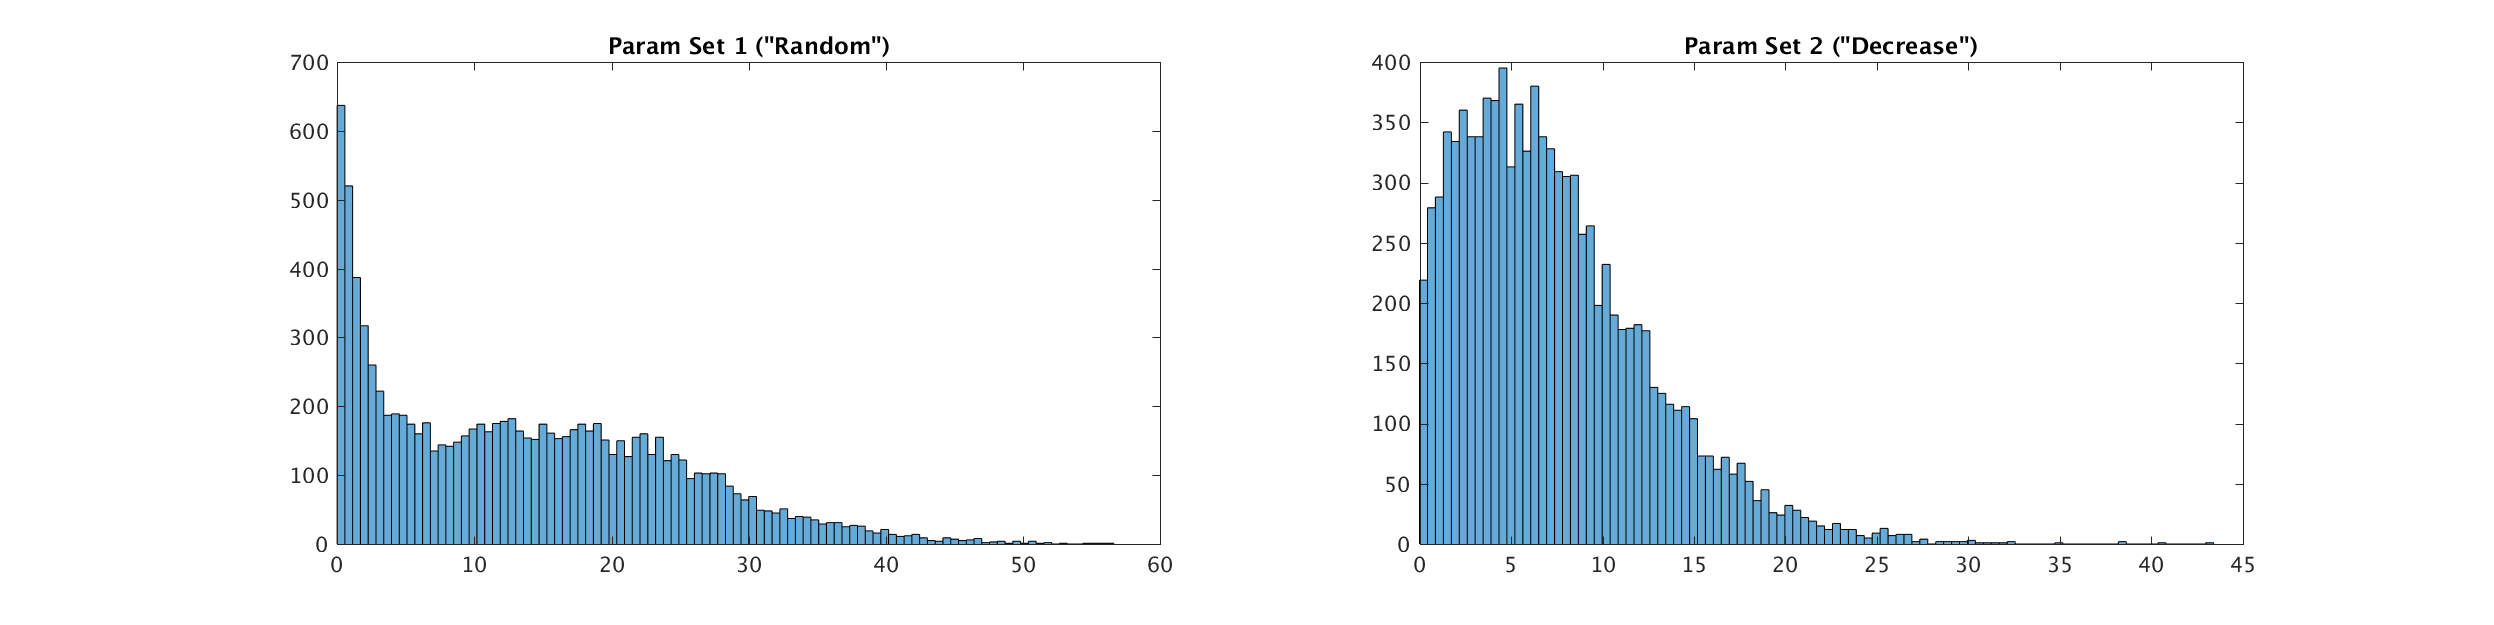
\includegraphics[width = \linewidth]{../model/steam/pic/random-decrease-time-compare-M-10000.eps}
		\caption{两组参数下用户停留时间直方图}\label{fig:random-decrease-time-compare-M-10000}
	\end{figure}

	参数推导的结果是良好的,在测试用户总体为 $M=10^4$ 的情况下能够通过优化获得 $5\%$ 的精度,已经能够满足精度上的要求。

	图 \ref{fig:random-decrease-score-compare-M-10000} 是依据推导出的参数进行打分的结果。可见总体趋势都是 $\text{Score}$ 随着 $x, \alpha$ 的增加而增加;而第一组参数随 $\alpha$ 的变动更为剧烈,这表示当项目的差异较大时,用户与用户间的体验差异可能较大。对比左右两种参数组,左边一组中相同的不满值 $x$ 对应的分数较大,表明参数组 1 可能更容易引起用户的不满。
	
	\begin{figure}[h!]
		\centering
		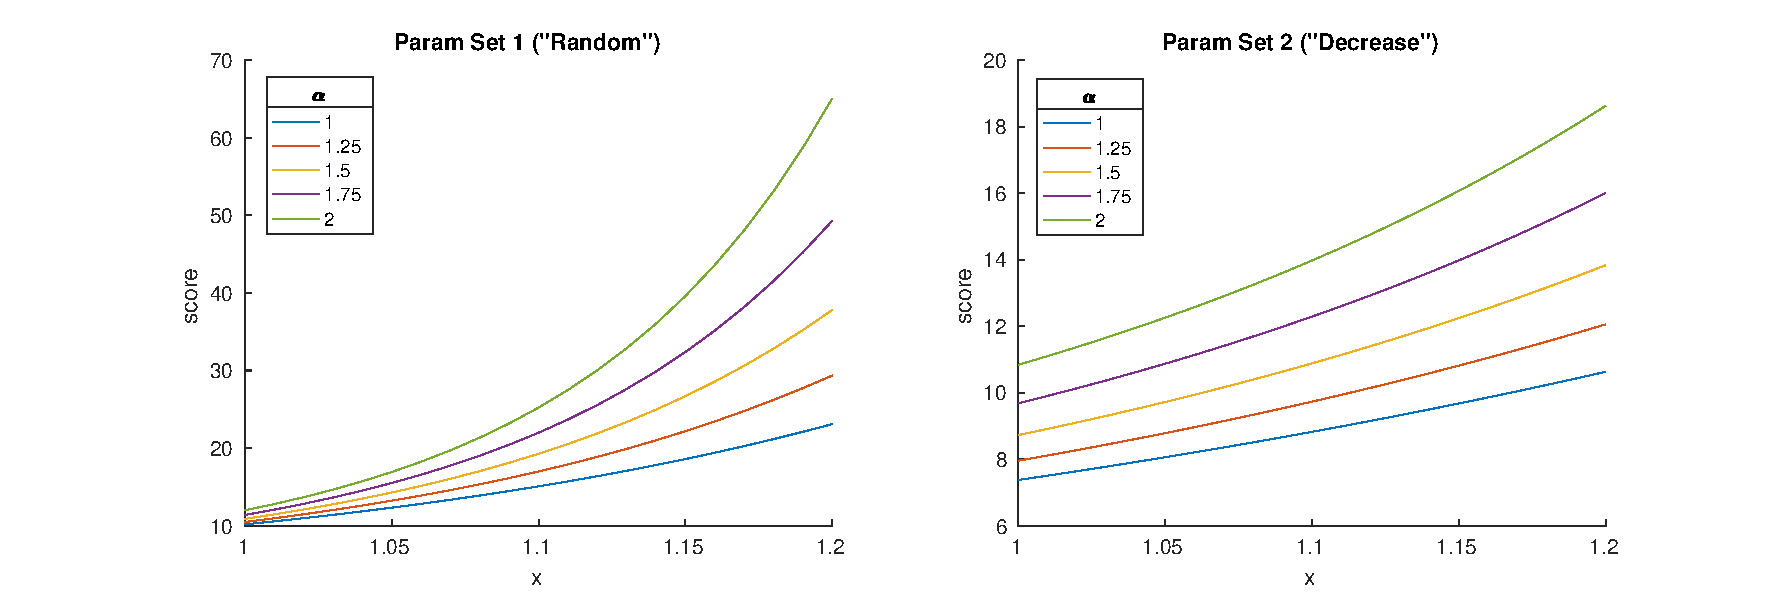
\includegraphics[width = \linewidth]{../model/steam/pic/random-decrease-score-compare-M-10000.eps}
		\caption{两组参数下推导出的$\mathrm{Score}_{\mathfrak{A}\left(\bm{\hat{\lambda}}, \bm{\hat{a}}, \omega\right)}(x, \alpha)$}\label{fig:random-decrease-score-compare-M-10000}
	\end{figure}
	
	
	\section{带跳过的顺序选择模型——美团、饿了吗外卖}
	\subsection{模型修正 \& 符号约定}
	在这一节中,我们考虑对第一个模型的修正——\textbf{带跳过的顺序选择模型}。\textbf{在这个模型中,每一个用户不必详细查看排行榜中的每一个产品,可以选择跳过其中的某些条目,只选择性的详细阅读某些条目。同无跳过的顺序选择模型一样,用户也必须且仅需做出一个选择}。这样的模型是基于美团、饿了吗外卖(\ref{modelB_fig_1})以及滴滴打车等一次性服务项目的功能简化得到的。
	\begin{figure}[h!]
		\centering
		
\includegraphics[width = 6cm]{modelB_fig_1.jpg}
		\caption{饿了吗外卖}\label{modelB_fig_1}
	\end{figure}
	
	例如上图,在使用饿了吗外卖时,用户会得到一个仅包含产品名的排行榜(我们认为得分也是排行榜的一部分,因此不予考虑)。用户会根据自己的经验或兴趣,顺着排行榜选择是否仔细阅读相关产品的信息;在发现自己想要的产品之后就做出选择。具体来说,我们给出带跳过的顺序模型修正后的定义。
	\begin{defn}\textbf{(带跳过的顺序选择模型)}该模型是一个建立在状态空间为$\mathcal{P} \cup \mathcal{\tilde{P}} \cup \left\{A\right\}$上的跳过程。其中$A$表示接受状态,$\mathcal{\tilde{P}}$表示判断是否要跳过状态$i \in \mathcal{P}$的状态。其中状态$i$处的指数闹钟参数为$\lambda_i$,在$\tilde{i}$处的指数闹钟参数为$\infty$,即瞬间跳跃;跳过状态$i$的概率为$s_i$,且其嵌入链的转移概率为
	\begin{equation}
	\begin{aligned}
	a_{p_N} & = 1 \\
	s_{p_N} & = 0 \\
	\bm{P}_{\tilde{p}_i, \tilde{p}_{i+1}} & = s_{p_i} \\
	\bm{P}_{\tilde{p}_i, p_i} & = 1 - s_{p_i} \\
	\bm{P}_{p_i,A}  & = a_{p_i} \\
	\bm{P}_{p_i,\tilde{p}_{i+1}} & = r_{p_i} = 1 - a_{p_i}
	\end{aligned}
	\end{equation}
	在图($\ref{modelB_fig_2}$)中展示了具体的模型。该模型可表述为$\mathfrak{B}\left(\bm{\lambda}, \bm{a}, \bm{s}, \omega\right)$。
	\end{defn}
	\begin{figure}[h!]
	\centering
	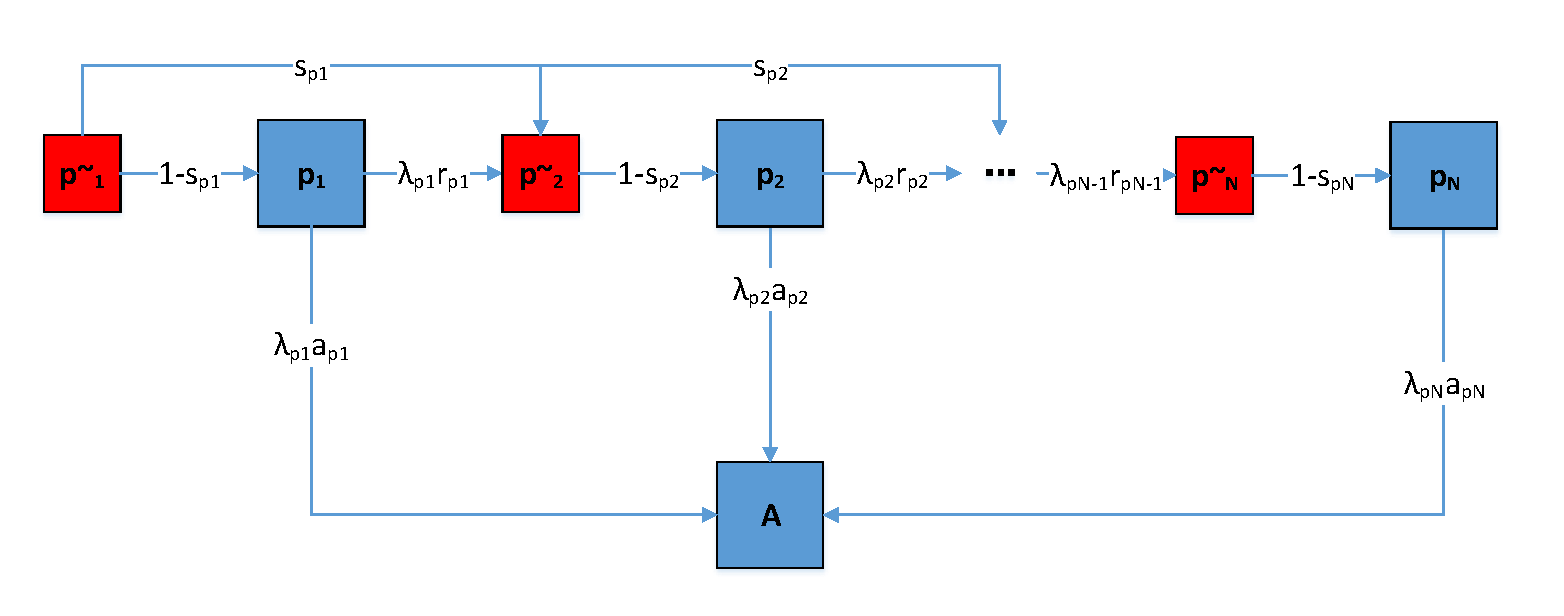
\includegraphics[width = 12cm]{modelB_fig_2.pdf}
	\caption{带跳过的顺序选择模型结构}\label{modelB_fig_2}
	\end{figure}
	
	\subsection{度量模型 \& 统计推断 \& 优化算法}
	与不带跳过的选择模型相同,我们依然选择用户找到其接受产品所花的时间$\tau_E$来衡量排行榜算法的优劣,并认为时间越短就越有效。同样的,我们可以得到
	\begin{equation} \label{EQ_B}
	\begin{aligned}
	\mathbb{E} \tau_E & = \sum_{k=1}^N \frac{(1-s_{p_j})\prod\limits_{j=0}^{k-1}(1-a_{p_j})}{\lambda_{p_i}} \\
	\mathrm{Var} \tau_E & = \sum_{k=1}^N (1-s_{p_j}^2)\left(\frac{\prod\limits_{j=0}^{k-1}(1-a_{p_j})}{\lambda_{p_i}}\right)^2
	\end{aligned}
	\end{equation}
	证明请参见附录。为了综合考虑期望和方差,我们用参数$\alpha$进行连续过渡;同样地,我们也使用指标$x$表示用户对于长队列的不满。综上,我们将衡量函数定义为
	\begin{equation}
	\mathrm{Score}_{\mathfrak{B}\left(\bm{\lambda}, \bm{a}, \bm{s}, \omega\right)} = \sum_{k=1}^N (1-s_{p_j})(1-s_{p_j}+\alpha s_{p_j})\left(\frac{\prod\limits_{j=0}^{k-1}(1-a_{p_j})}{\lambda_{p_i}} x^k\right)^\alpha, \quad x \in [1, \infty], \alpha \in [1, 2]
	\end{equation}
	相应的,参数$\bm{\lambda}, \bm{a}, \bm{s}$均是隐含的,我们需要从数据中学习出这些参数的推断值$\bm{\hat{\lambda}}, \bm{\hat{a}}, \bm{\hat{s}}$,然后再代入上式进行计算。依然使用似然函数的办法和优化策略解决这个问题。
	\subsection{实验结果}
	同样的,我们生成了两组参数来生成不同的数据,参见表 \ref{tab:meituan-param} 。
	
	\begin{table}[h!]
		\tiny
		\centering
		\label{tab:meituan-param}
		\begin{tabular}{cc|cccccccccc|c}
			\hline
			&                                         & 1 & 2 & 3 & 4 & 5 & 6 & 7 & 8 & 9 & 10 & $\epsilon_{\text{rel}}$\\
			\hline
			\multirow{4}{*}{Set 1 \textbf{Random}}
			& $\lambda$       & 0.896 & 0.489 & 0.894 & 0.595 & 0.398 & 0.956 & 0.690 & 0.476 & 0.656 & 0.417 & \multirow{2}{*}{1.9525e-01} \\
			& $\hat{\lambda}$ & 1.026 & 0.507 & 1.077 & 0.672 & 0.483 & 0.994 & 0.741 & 0.664 & 0.915 & 0.479 & \\
			& $a$             & 0.782 & 0.839 & 0.821 & 0.860 & 0.834 & 0.983 & 0.956 & 0.955 & 0.980 & \slash& \multirow{2}{*}{9.2899e-04} \\
			& $\hat{a}$       & 0.782 & 0.838 & 0.823 & 0.861 & 0.835 & 0.984 & 0.955 & 0.955 & 0.979 & \slash& \\
			& $s$             & 0.126 & 0.043 & 0.173 & 0.117 & 0.170 & 0.035 & 0.066 & 0.286 & 0.279 & 0.126 & \multirow{2}{*}{7.2698e-01} \\
			& $\hat{s}$       & 0.158 & 0.051 & 0.202 & 0.135 & 0.199 & 0.035 & 0.068 & 0.297 & 0.285 & 0.500 & \\
			\hline
			\multirow{4}{*}{Set 2 \textbf{Decrease}}
			& $\lambda$       & 0.500 & 0.500 & 0.500 & 0.500 & 0.500 & 0.500 & 0.500 & 0.500 & 0.500 & 0.500 & \multirow{2}{*}{3.3464e+00} \\
			& $\hat{\lambda}$ & 0.500 & 0.557 & 0.631 & 0.709 & 0.835 & 1.018 & 1.242 & 1.663 & 2.630 & 5.095 & \\
			& $a$             & 0.900 & 0.800 & 0.700 & 0.600 & 0.500 & 0.400 & 0.300 & 0.200 & 0.100 & \slash& \multirow{2}{*}{5.2407e-03} \\
			& $\hat{a}$       & 0.899 & 0.798 & 0.701 & 0.603 & 0.496 & 0.402 & 0.300 & 0.196 & 0.095 & \slash& \\
			& $s$             & 0.000 & 0.100 & 0.200 & 0.300 & 0.400 & 0.500 & 0.600 & 0.700 & 0.800 & 0.900 & \multirow{2}{*}{3.6854e-01} \\
			& $\hat{s}$       & 0.000 & 0.123 & 0.264 & 0.412 & 0.573 & 0.713 & 0.832 & 0.922 & 0.977 & 0.500 & \\
			\hline
		\end{tabular}
		\caption{有跳过的顺序选择模型的参数选择}
	\end{table}
	\normalsize
	
	可见,除了第二组的 $\hat{\lambda}$ 外,其余预测均较为准确(一个可能的原因是在有跳过之后用户有效阅读次数下降,导致需要更多的样本才能拟合到较为准确的数据)。
	
	同样的,我们可以对比不同参数下用户的停留时间、每个项目的被呈现且跳过的概率和排行榜最终得分。
	
	\begin{figure}[h!]
		\centering
		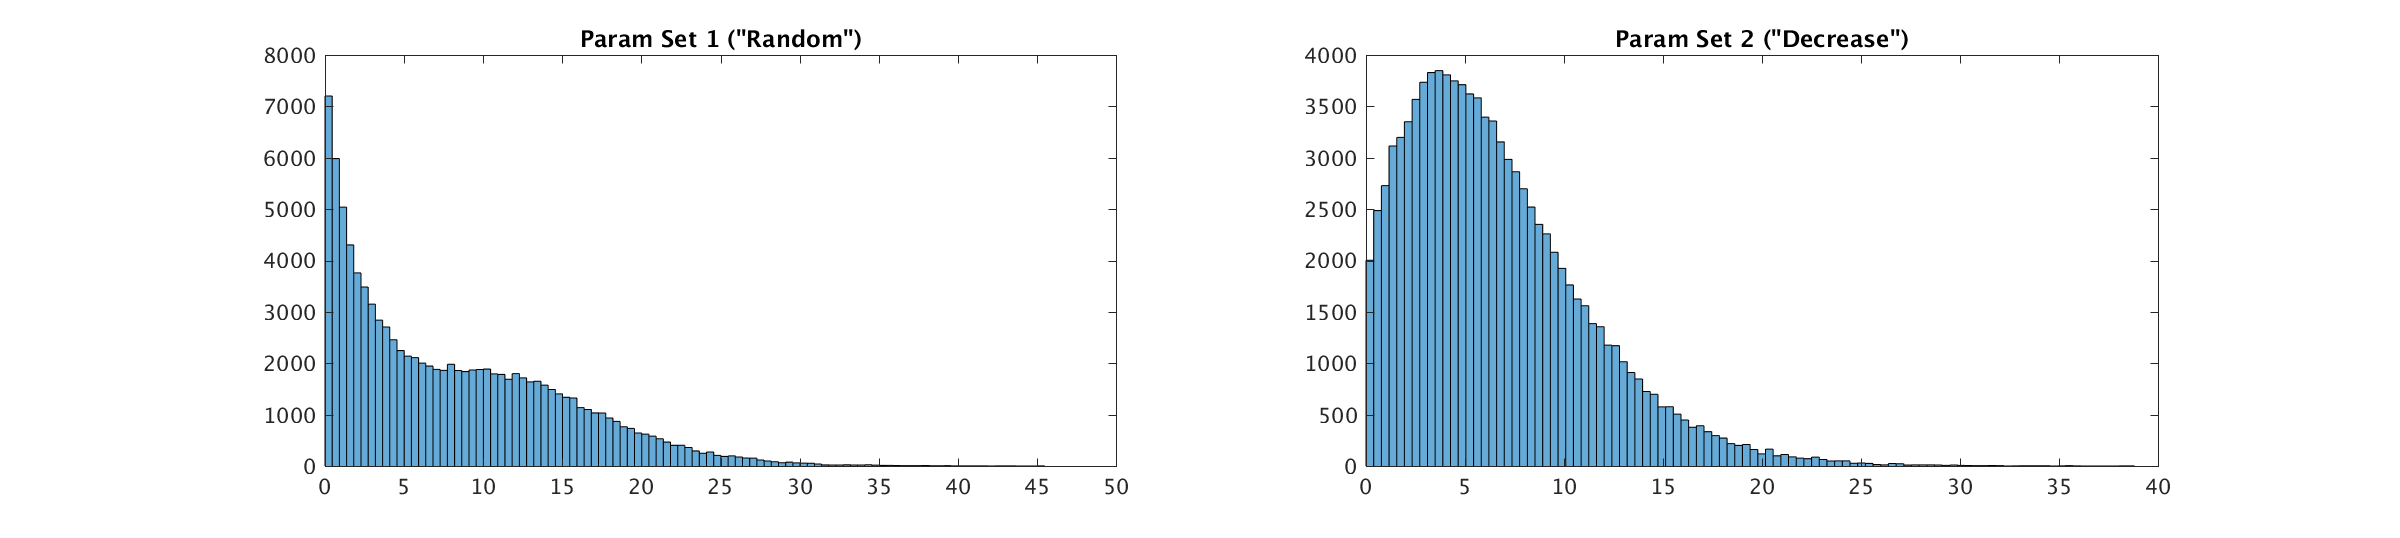
\includegraphics[width = \linewidth]{../model/meituan/pic/random-decrease-time-compare-M-100000.eps}
		\caption{两组参数下用户停留时间直方图}\label{fig:random-decrease-time-compare-M-100000}
	\end{figure}

	可见参数组 1 与 2 表现出截然不同的停留时间分布。同样的,用户跳过项目的概率也会呈现出不同的模式:在参数组 2 中我们通过随项目推进不断增大的退出概率和不断增大的跳过概率来达到某种平衡,使得越靠后的项目被呈现概率越低——同时它们被跳过的概率也就越高。

	\begin{figure}[h!]
		\centering
		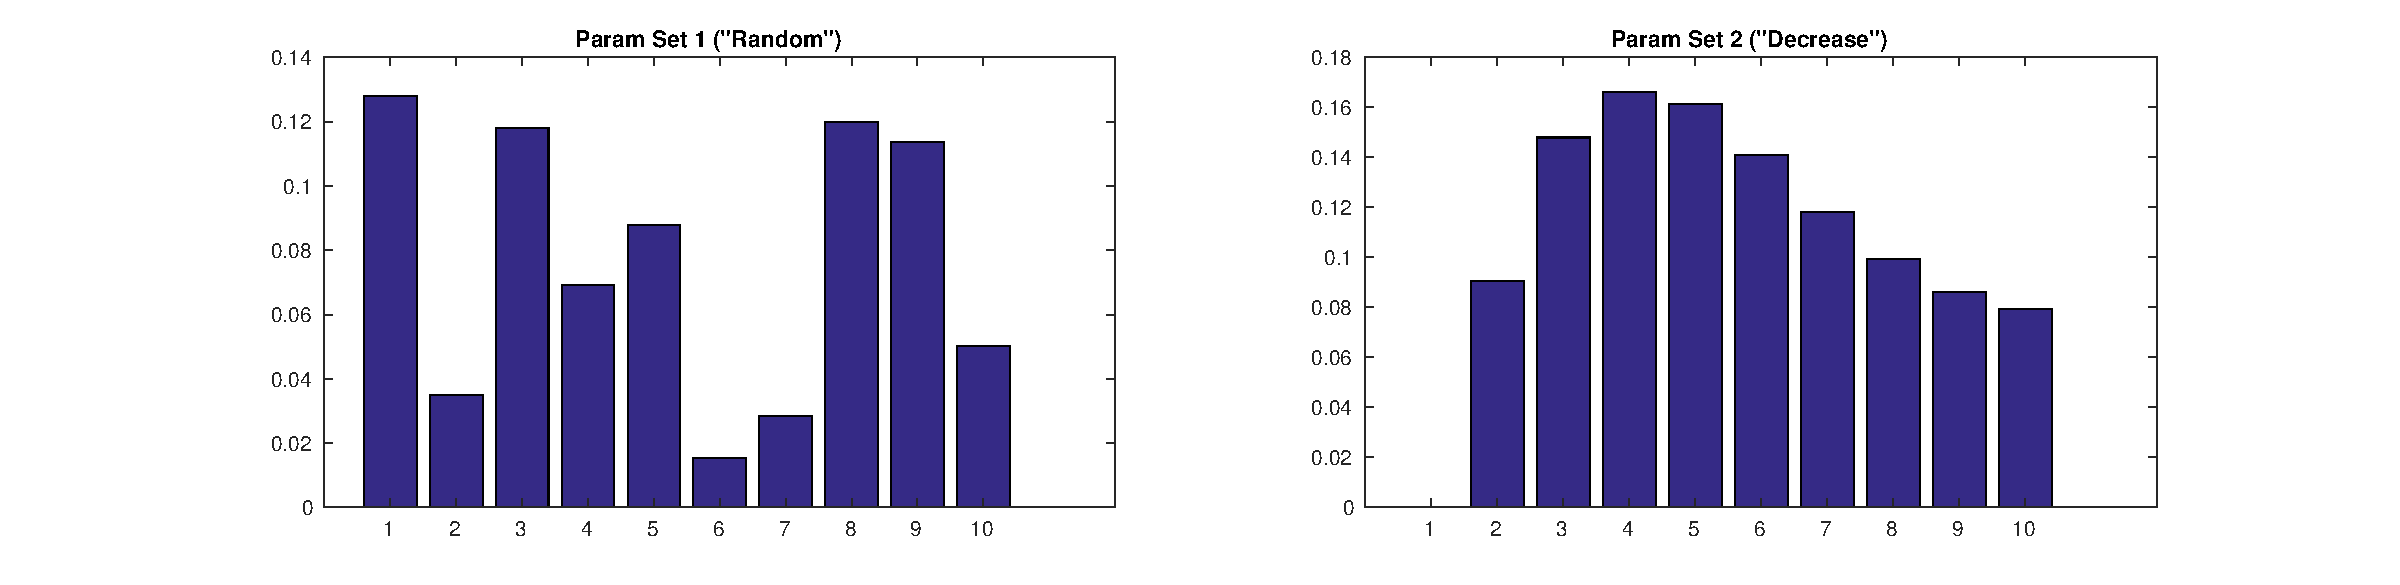
\includegraphics[width = \linewidth]{../model/meituan/pic/random-decrease-skip-compare-M-100000.eps}
		\caption{两组参数下用户跳过每个项目概率直方图}\label{fig:random-decrease-skip-compare-M-100000}
	\end{figure}

	接下来我们需要验证我们给出的 Score 是否合理:通过比较两个参数组给出的分数随 $x, \alpha$ 变化图线 \ref{fig:random-decrease-score-compare-M-100000} 可知,随机参数受 $x, \alpha$ 变化的影响更大,这意味着如果我们设置了较小的 $x$ 或 $\alpha$,可能就无法估计到一部分焦躁客户的感受。
	
	\begin{figure}[h!]
		\centering
		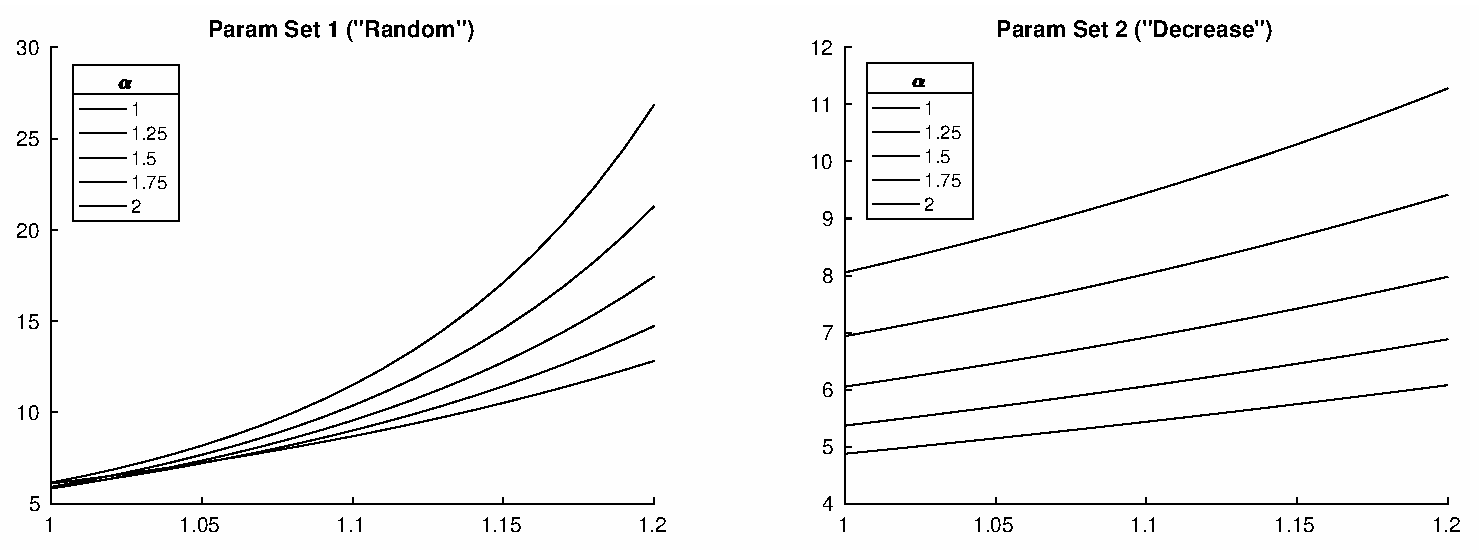
\includegraphics[width = \linewidth]{../model/meituan/pic/random-decrease-score-compare-M-100000.eps}
		\caption{两组参数下推导出的$\mathrm{Score}_{\mathfrak{A}\left(\bm{\hat{\lambda}}, \bm{\hat{a}}, \omega\right)}(x, \alpha)$}\label{fig:random-decrease-score-compare-M-100000}
	\end{figure}
	
	\section{带跳过的投票模型——豆瓣、知乎推荐}
	\subsection{模型修正 \& 符号约定}
    本节中,我们考虑一个与前两种模型有一定差异的模型——\textbf{带跳过的投票模型}。在此模型中,用户浏览条目的目的不再是为了接受其中的一个,而是为了单纯获得阅读体验。\textbf{用户对每一个条目进行结果为赞成、反对或是不表态的投票,同时每一个用户不必详细查看排行榜中的每一个产品,可以选择跳过其中的某些条目,只选择性的详细阅读某些条目。用户不必须阅读至列表结尾,而是可以在中间时刻选择结束}。这样的模型是基于豆瓣、知乎的论坛类应用的推荐功能简化得到的。
	\begin{defn}\textbf{(带跳过的投票模型)}该模型是一个建立在状态空间为$\mathcal{P} \cup \mathcal{\tilde{P}} \cup \mathcal{U} \cup \mathcal{D} \cup \mathcal{N} \cup \left\{T\right\}$上的跳过程。其中$T$表示结束状态,$\mathcal{\tilde{P}}$表示判断是否要跳过状态$i \in \mathcal{P}$的状态,$\mathcal{U}$表示第$i$个状态的结果为\textbf{赞成}的状态,$\mathcal{D}$表示第$i$个状态的结果为\textbf{反对}的状态,$\mathcal{N}$表示第$i$个状态的结果为\textbf{不予评价}的状态。其中状态$i$处的指数闹钟参数为$\lambda_i$,在$\tilde{i}$以及$\mathcal{U}$,$\mathcal{D}$,$\mathcal{N}$所对应状态处的指数闹钟参数为$\infty$,即瞬间跳跃;跳过状态$i$的概率为$s_i$,若不跳过则赞成的概率为$u_i$,反对的概率为$d_i$,不予评价的概率为$n_i$;且其嵌入链的转移概率为
	\begin{equation}
	\begin{aligned}
	a_{p_N} & = 1 \\
	s_{p_N} & = 0 \\
	\bm{P}_{\tilde{p}_i, \tilde{p}_{i+1}} & = s_{p_i} \\
	\bm{P}_{\tilde{p}_i, p_i} & = 1 - s_{p_i} \\
	\bm{P}_{p_i,T}  & = t_{p_i} \\
	\bm{P}_{p_i,u_i} & = u_i \\
	\bm{P}_{p_i,d_i} & = d_i \\
	\bm{P}_{p_i,n_i} & = n_i \\
	u_i + d_i + n_i & = 1\\
	\bm{P}_{u_i, \tilde{p}_{i+1}} & = \bm{P}_{d_i, \tilde{p}_{i+1}} = \bm{P}_{n_i, \tilde{p}_{i+1}} = 1 \\
	\bm{P}_{u_N, T} & = \bm{P}_{d_N, T} = \bm{P}_{n_N, T} = 1
	\end{aligned}
	\end{equation}
	这里和后面都会用$u_i,d_i,n_i$同时表示概率和状态的含义,在表达式中不会产生歧义。在图($\ref{modelC_fig_2}$)中展示了具体的模型。该模型可表述为$\mathfrak{C}\left(\bm{\lambda}, \bm{t}, \bm{s}, \bm{u}, \bm{d}, \bm{n},\omega\right)$。
	\end{defn}
	\begin{figure}[h!]
		\centering
		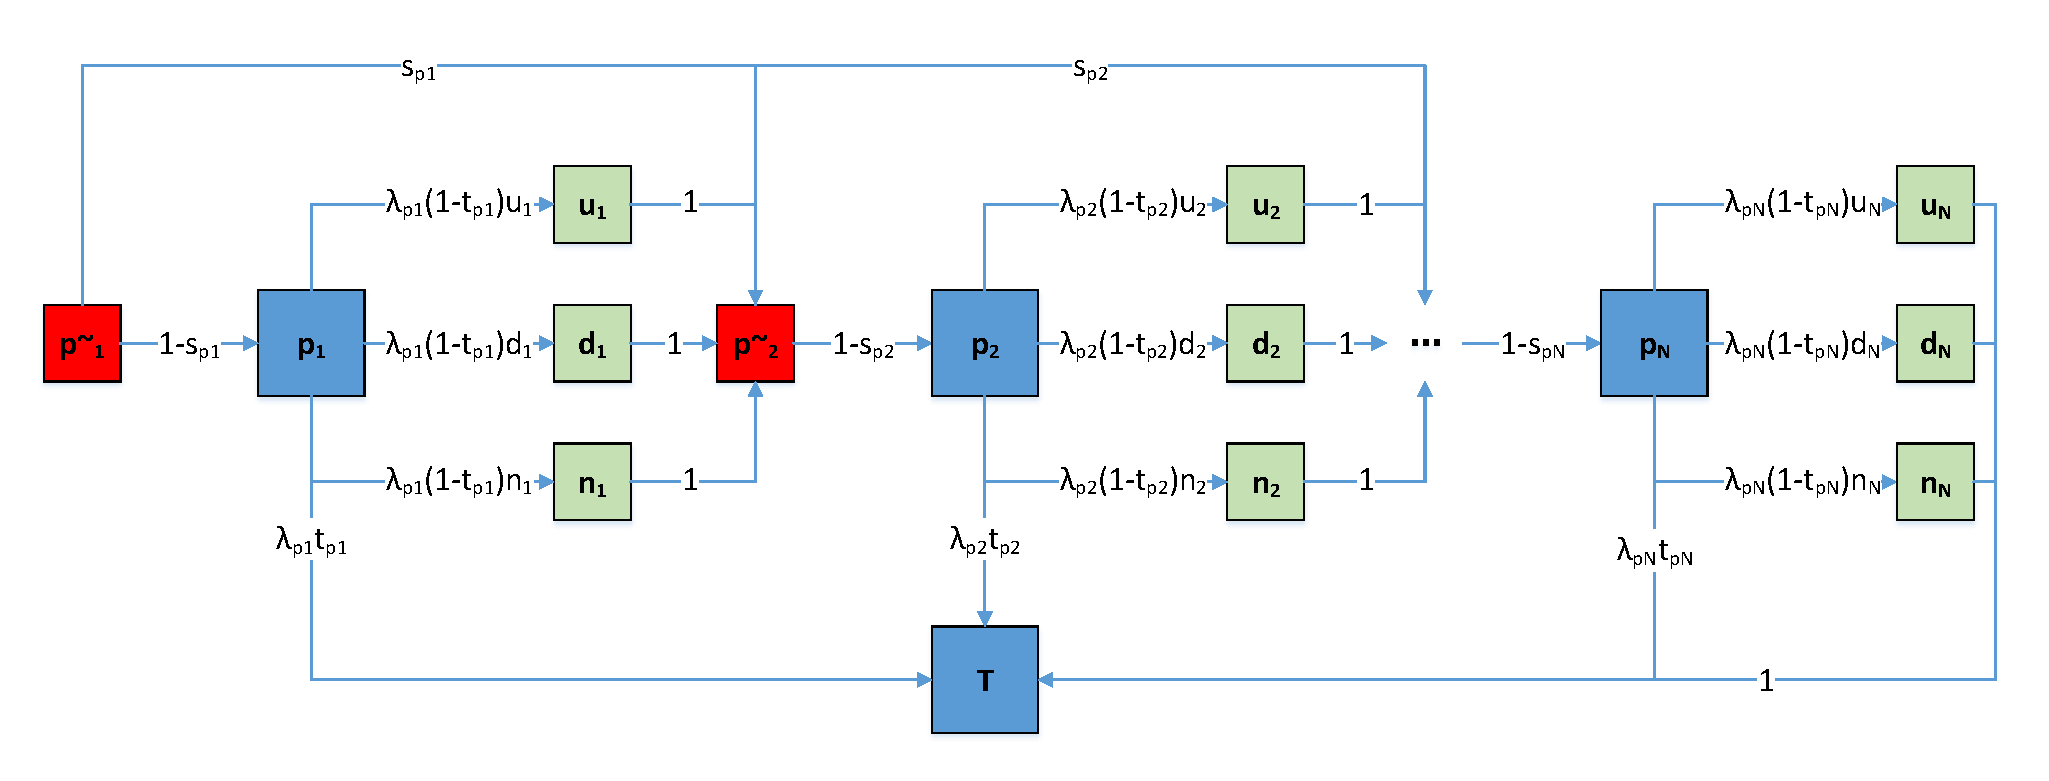
\includegraphics[width = 12cm]{modelC_fig_2.pdf}
		\caption{带跳过的投票模型结构}\label{modelC_fig_2}
	\end{figure}
	
	\subsection{度量模型 \& 统计推断 \& 优化算法}
	在这里,我们用一种新定义的\textbf{有效体验时间}$\tau_T$来衡量排行榜的好坏。具体来说$\tau_T$是\textbf{所有做出了赞成或反对的阅读时间的总和}。对于豆瓣、知乎这种阅读体验累的产品来说,用户能够对阅读的产品更长时间的保持兴趣则产品设计的越好,而在阅读完之后做出了赞成或反对的选择就表示用户对于这个条目很感兴趣,这段时间可以被看作是有效的。具体来说,我们可以计算出$\tau_T$的期望和方差为
	\begin{equation} \label{EQ_C}
	\begin{aligned}
	\varphi_{p_j} & = s_{p_j} + n_{p_j} - s_{p_j}n_{p_j} \\
	\mathbb{E} \tau_T & = \sum_{k=1}^N \frac{(1-\varphi_{p_j})\prod\limits_{j=0}^{k-1}(1-t_{p_j})}{\lambda_{p_i}} \\
	\mathrm{Var} \tau_T & = \sum_{k=1}^N (1-\varphi_{p_j}^2)\left(\frac{\prod\limits_{j=0}^{k-1}(1-t_{p_j})}{\lambda_{p_i}}\right)^2
	\end{aligned}
	\end{equation}
	证明请参见附录。为了综合考虑期望和方差,我们用参数$\alpha$进行连续过渡;同样地,我们也使用指标$x$表示用户对于后面才出现的感兴趣的话题不满。综上,我们将衡量函数定义为
	\begin{equation}
	\mathrm{Score}_{\mathfrak{C}\left(\bm{\lambda}, \bm{t}, \bm{s}, \bm{u}, \bm{d}, \bm{n},\omega\right)} = \sum_{k=1}^N (1-\varphi_{p_j})(1-\varphi_{p_j}+\alpha \varphi_{p_j})\left(\frac{\prod\limits_{j=0}^{k-1}(1-t_{p_j})}{\lambda_{p_i}} x^k\right)^\alpha, \quad x \in (0, 1], \alpha \in [1, 2]
	\end{equation}
	相应的,参数$\bm{\lambda}, \bm{t}, \bm{s}, \bm{u}, \bm{d}, \bm{n}$均是隐含的,我们需要从数据中学习出这些参数的推断值$\bm{\hat{\lambda}}, \bm{\hat{t}}, \bm{\hat{s}}, \bm{\hat{u}}, \bm{\hat{d}}, \bm{\hat{n}}$,然后再代入上式进行计算。依然使用似然函数的办法和优化策略解决这个问题。 \\
	
	注意到,与上面的情况不同,我们的这个衡量函数实际上是在测量用户的\textbf{有效体验时间},因此$\mathrm{Score}_{\mathfrak{C}\left(\bm{\hat{\lambda}}, \bm{\hat{t}}, \bm{\hat{s}}, \bm{\hat{u}}, \bm{\hat{d}}, \bm{\hat{n}},\omega\right)}$的越大我们认为排行榜越好。
	
	我们将这一部分的数值实验放在下一节中进行展示与分析。
	
	\section{实时计算}
	由于排行榜具有很强的时效性和话题性,除非是一些长久建立的口碑排行榜(如旅游景点排行榜),我们在推断产品固有性质中的$a_i,r_i,s_i,t_i,u_i,d_i,n_i$时都不能把他们当做常数看待,而应该把它们都看做关于时间$t$的函数。因此,在推断某个时刻$t$的产品固有性质的值时,我们可以将所有$[t-\Delta t,t)$内的用户作为有效数据点来进行推测。$\Delta t$的选择应该适中,使得用户样本量足够大且间隔不会太长使得推断的结果不够准。
	\section{实际产品评价}
    本节中,我们将对两种著名的排行榜产品——\textbf{Hacker News ranking algorithm}以及\textbf{Reddit ranking algorithms}进行介绍,并利用我们上面的第五节中得到的模型对其进行评价、比较。通过对这两种排行榜产品的实验,验证上述衡量函数的合理性。
	\subsection{两种著名的排行榜产品}
    这两种排行榜产品均适用于上述带跳过的投票模型,通过对每一条目所得赞同数$U$与反对数$D$以及该条目的发出时间$T$进行分析,从而得出单个条目的得分$\mathrm{Score}$。再根据$\mathrm{Score}$从大到小排序得出排行榜。具体$\mathrm{Score}$函数定义分别如下:

    \begin{itemize}
        \item \textbf{Hacker News ranking algorithm}\footnote{\url{https://medium.com/hacking-and-gonzo/how-hacker-news-ranking-algorithm-works-1d9b0cf2c08d}}
        \begin{equation}
        \begin{aligned}
        P & = U - D \\
	    \mathrm{Score} & = (P - 1)/(T + 2)^G
        \end{aligned}
	    \end{equation}
        其中$G$为重力参数,默认值为1.8。
        \item \textbf{Reddit ranking algorithms}\footnote{\url{https://medium.com/hacking-and-gonzo/how-reddit-ranking-algorithms-work-ef111e33d0d9}}
        \begin{equation}
        \begin{aligned}
        t_{s} & = -t \\
        P & = U - D \\
        Q & = \begin{cases}
                1, \quad \mathrm{if} \ P > 0 \\
                0, \quad \mathrm{if} \ P = 0 \\
                -1, \quad \mathrm{if} \ P < 0
            \end{cases} \\
        R & = \begin{cases}
            |P|, \quad \mathrm{if} \ |P| \geq 1 \\
            1, \quad \mathrm{if} \ |P| < 1
            \end{cases} \\
        \mathrm{Score} & =  \log_{10} R + \frac{Qt_s}{45000}
        \end{aligned}
	    \end{equation}
    \end{itemize}
    可以看出,这两种方法下均是较新的、发布时间较短的条目更容易排名靠前(这点也符合一般的实际情况)。区别只是随着时间的推移Hacker News ranking algorithm下的$\mathrm{Score}$将会下降,而Reddit ranking algorithms下的$\mathrm{Score}$不一定会下降,但是新条目的得分往往高于旧条目。这说明这两种方法均有一定的合理性。

	\subsection{不同情形下的实验比较}
	首先我们设定参数的生成:考虑时间 $t$ 以天为单位,那么我们可以不妨假设参数依赖于每天的时刻,那么可以做出如下的设定:
	\begin{align}
		\lambda &= \cos(2\pi(t+0.1)) \cdot 0.4 + 1 \\
		s &= \cos(2\pi(t+0.8)) \cdot 0.05 + 0.1 \\
		t &= \cos(2\pi(t+0.4))\cdot 0.06 + 0.1 \\
		u &= (\cos(2\pi(t+0.3)) \cdot 0.2 + 0.5)(\cos(2\pi(t+0.5))\cdot 0.1 + 0.5) \\
		d &= (-\cos(2\pi(t+0.3)) \cdot 0.2 + 0.5)(\cos(2\pi(t+0.5))\cdot 0.1 + 0.5)
	\end{align}
	
	在这种参数的设置下,我们考虑已经生成了 19 篇带有如上规律参数的文章,我们模拟用户的访问、评价等操作,并及时更新排行榜以影响到之后的用户。
	
	首先我们关注两种算法下用户停留时间与跳过条目的概率,以及排行榜评价分数随 $x, \alpha$ 的变化规律:
	
	\begin{figure}[h!]
		\centering
		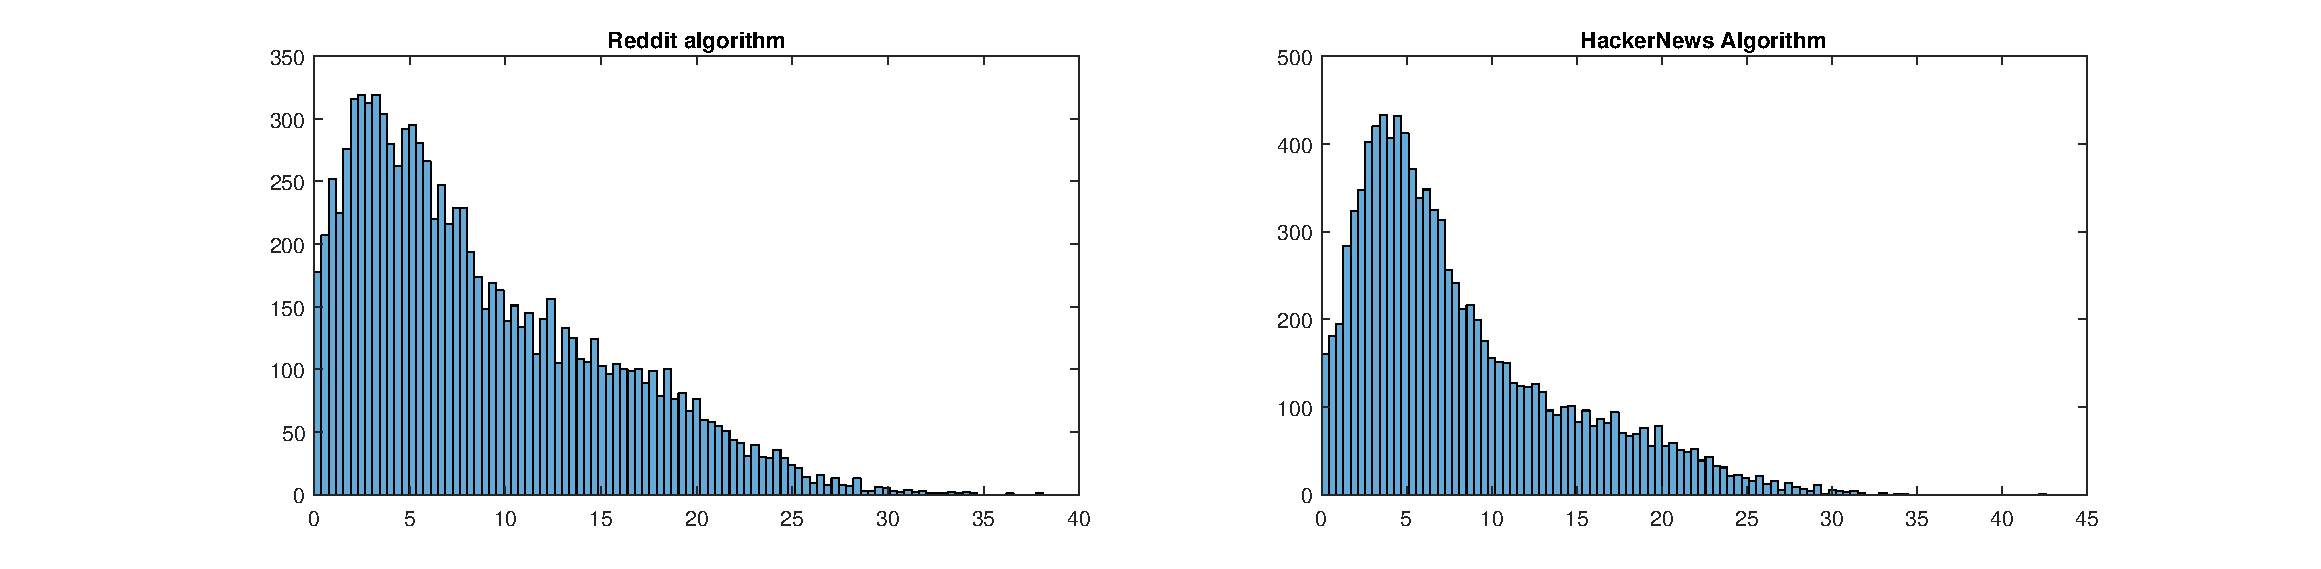
\includegraphics[width = \linewidth]{../model/douhu/pic/reddit-h-time.eps}
		\caption{两种算法下用户停留时间直方图}\label{fig:reddit-h-time}
	\end{figure}
	
	相较而言, HackerNews 算法给出的停留时间分布具有更窄的尖峰,均值也较小;而跳过概率直方图在两个算法方案下表现较为一致,基本都是前面的容易跳过。
	
	\begin{figure}[h!]
		\centering
		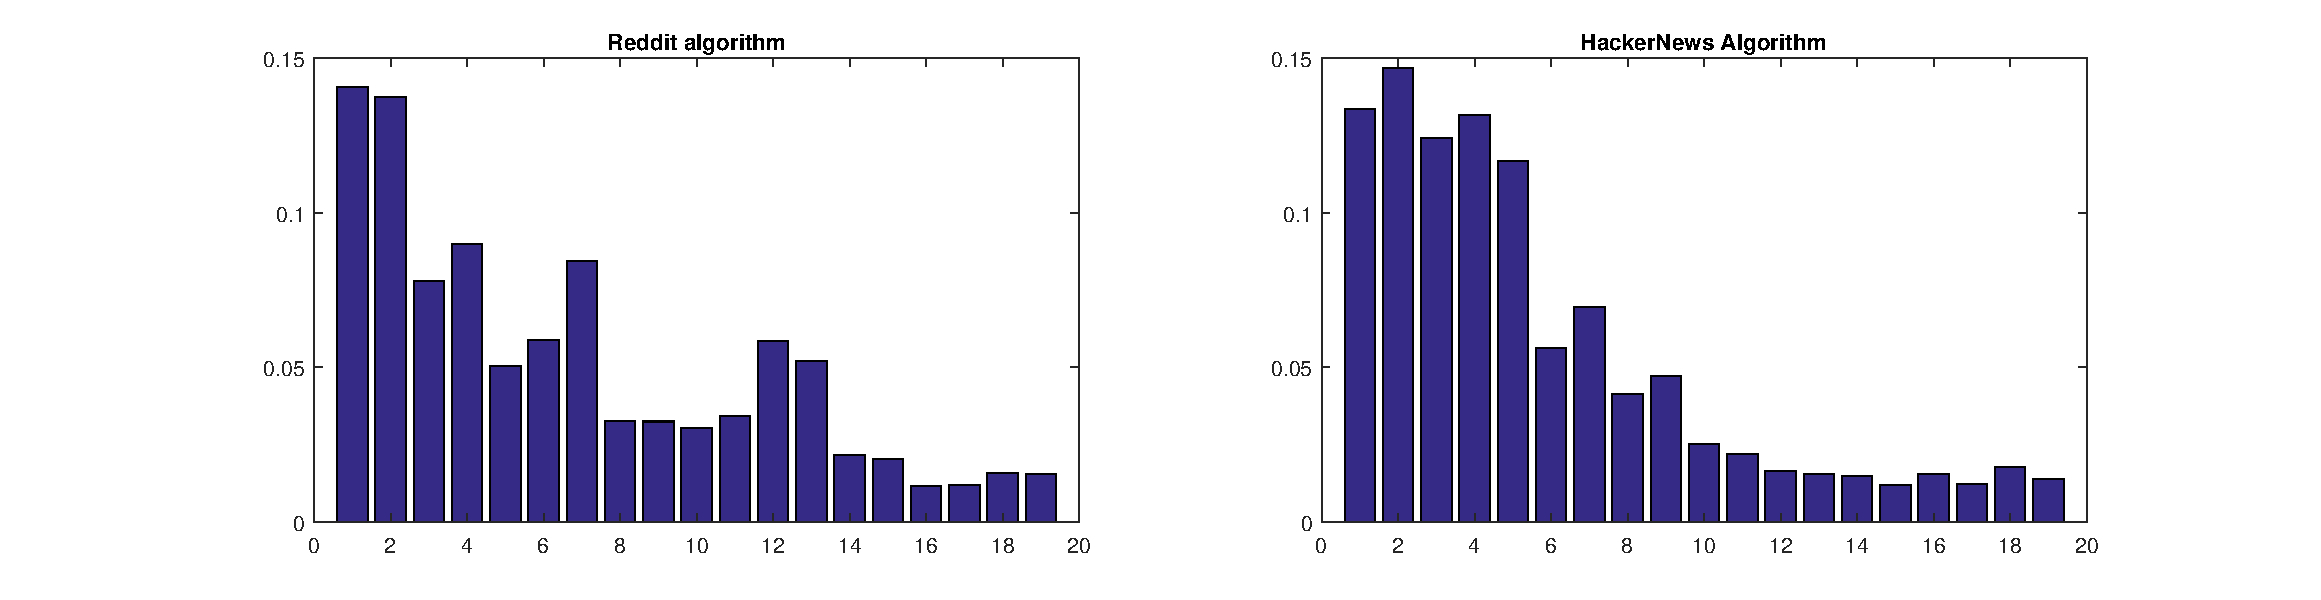
\includegraphics[width = \linewidth]{../model/douhu/pic/reddit-h-skip.eps}
		\caption{两种算法下用户跳过每个项目概率直方图}\label{fig:reddit-h-skip}
	\end{figure}
	
	接下来我们仍需要验证我们给出的 Score 是否合理:通过比较两个算法给出的分数随 $x, \alpha$ 变化图线 \ref{fig:reddit-h-score} 可知,Reddit 算法受 $x, \alpha$ 变化的影响更大,这意味着 Reddit 的重度用户可能更加能够享受到推荐算法带来的快乐。
	
	\begin{figure}[h!]
		\centering
		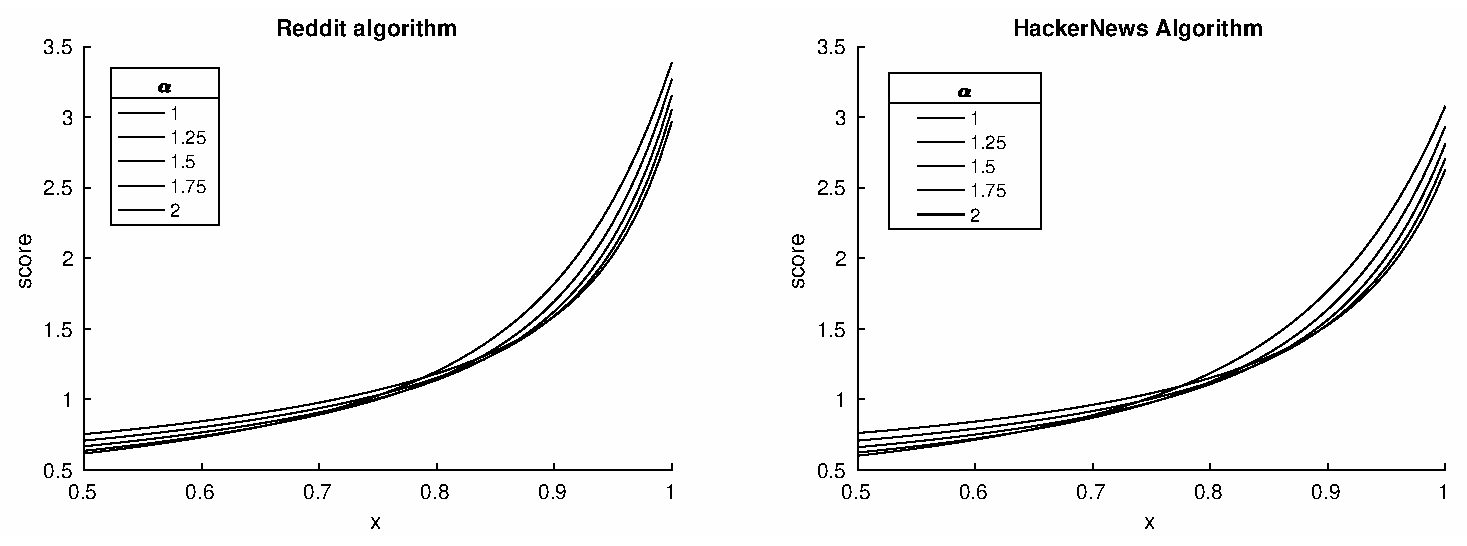
\includegraphics[width = \linewidth]{../model/douhu/pic/reddit-h-score.eps}
		\caption{两种算法下推导出的$\mathrm{Score}_{\mathfrak{C}\left(\bm{\hat{\lambda}}, \bm{\hat{t}}, \bm{\hat{s}}, \bm{\hat{u}}, \bm{\hat{d}}, \bm{\hat{n}},\omega\right)}$}\label{fig:reddit-h-score}
	\end{figure}
	
	\section{由此启发得到的基于优化的排行榜算法}
	尽管不是题目所要求的,但我们很容易注意到通过得到的费用函数,我们可以得到一个由此启发的排行榜算法,即
	\begin{equation}
	\hat{\omega} = \argmax_{\omega \in \Omega_P} \mathrm{Score}_{\mathfrak{C}\left(\bm{\hat{\lambda}}, \bm{\hat{t}}, \bm{\hat{s}}, \bm{\hat{u}}, \bm{\hat{d}}, \bm{\hat{n}},\omega\right)}
	\end{equation}
	其中推断得到的参数$\bm{\hat{\lambda}}, \bm{\hat{t}}, \bm{\hat{s}}, \bm{\hat{u}}, \bm{\hat{d}}, \bm{\hat{n}}$是实时计算的。 \\
	
	注意到这样一个优化问题是非凸的组合优化问题,且搜索空间大小为$|\Omega_P| = N! \sim \sqrt{2\pi N} \left(N/e\right)^N$,不可能遍历搜索。我们采用贪心的策略,从一个随机的排列出发,遍历两两交换下所能使函数值提升最大的$\omega$并迭代更新,具体来说迭代法为
	$$
	\omega_{n+1} =  \argmax_{|\omega - \omega_n| = 1} \mathrm{Score}_{\mathfrak{C}\left(\bm{\hat{\lambda}}, \bm{\hat{t}}, \bm{\hat{s}}, \bm{\hat{u}}, \bm{\hat{d}}, \bm{\hat{n}},\omega\right)}
	$$
	其中$|\omega_1 -\omega_2|$表示至少通过多少步两两交换能够将$\omega_1$变为$\omega_2$,这显然是$\Omega_P$上的一个距离。下面我们将此排行榜算法与Hacker News和Reddit排行榜算法进行比较,得到的数值实验结果如下。
	
	首先我们观察不同算法给出的排行榜热力图的形状:
	\begin{figure}[h!]
		\centering
		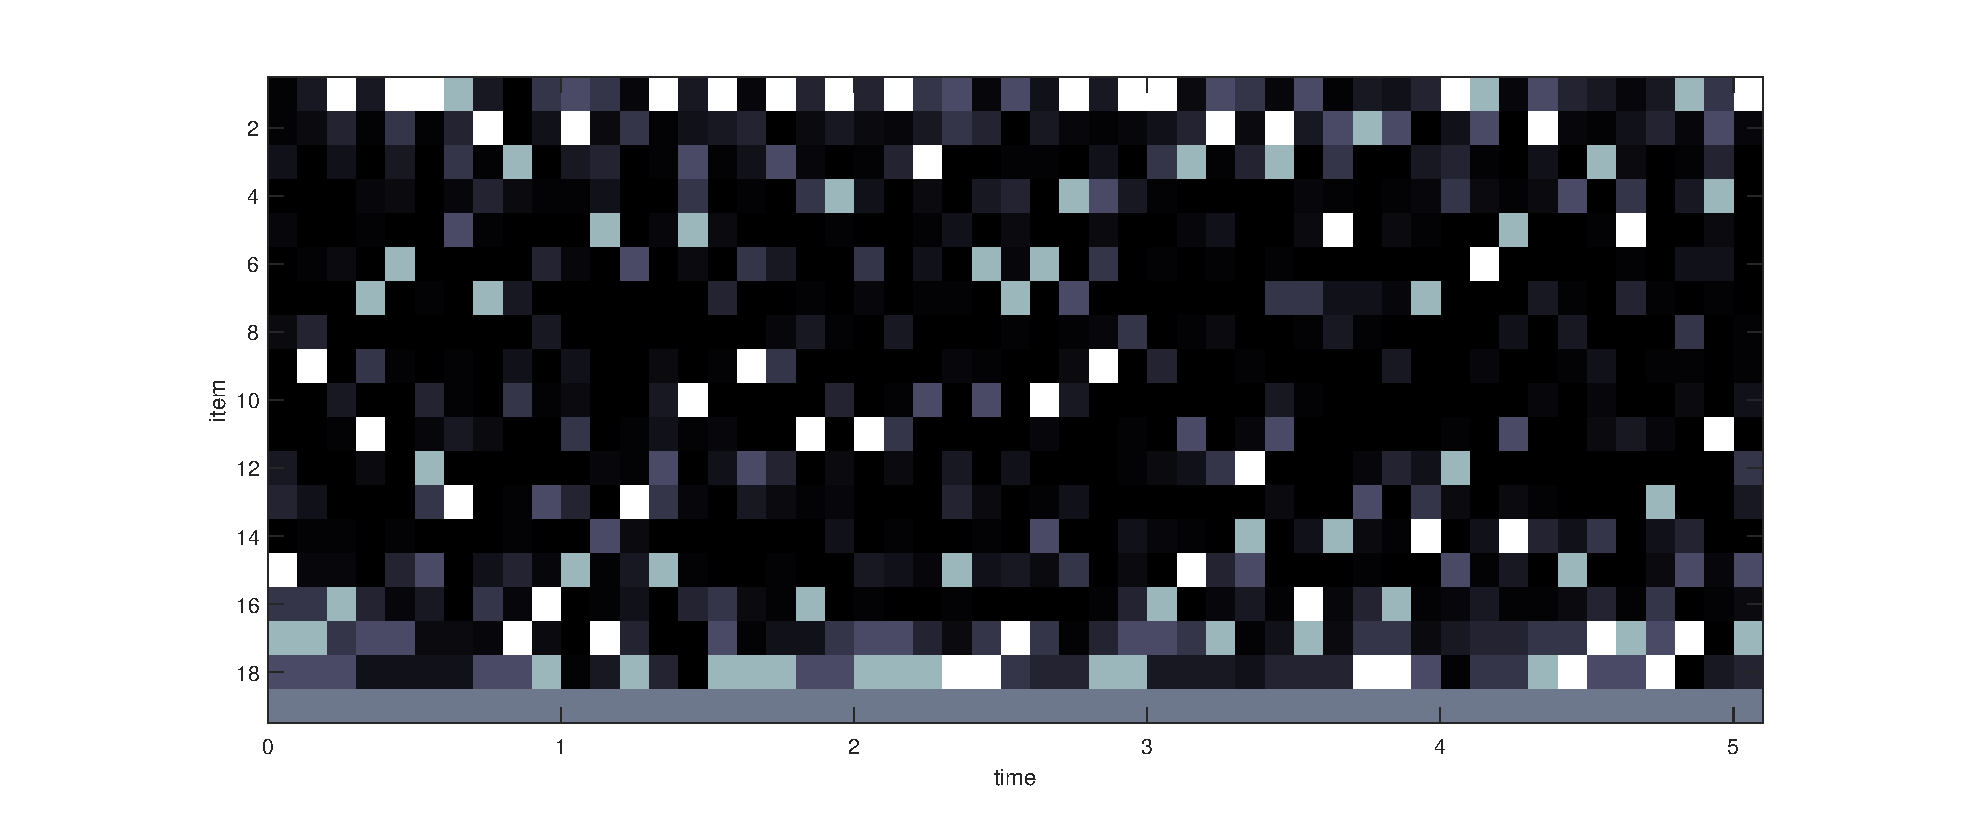
\includegraphics[width = \linewidth]{../model/douhu/pic/reddit-heatmap.eps}
		\caption{Reddit 算法给出的排行榜演化, $x=0.5, \alpha=1.5$}\label{fig:reddit-heatmap}
	\end{figure}

	\begin{figure}[h!]
		\centering
		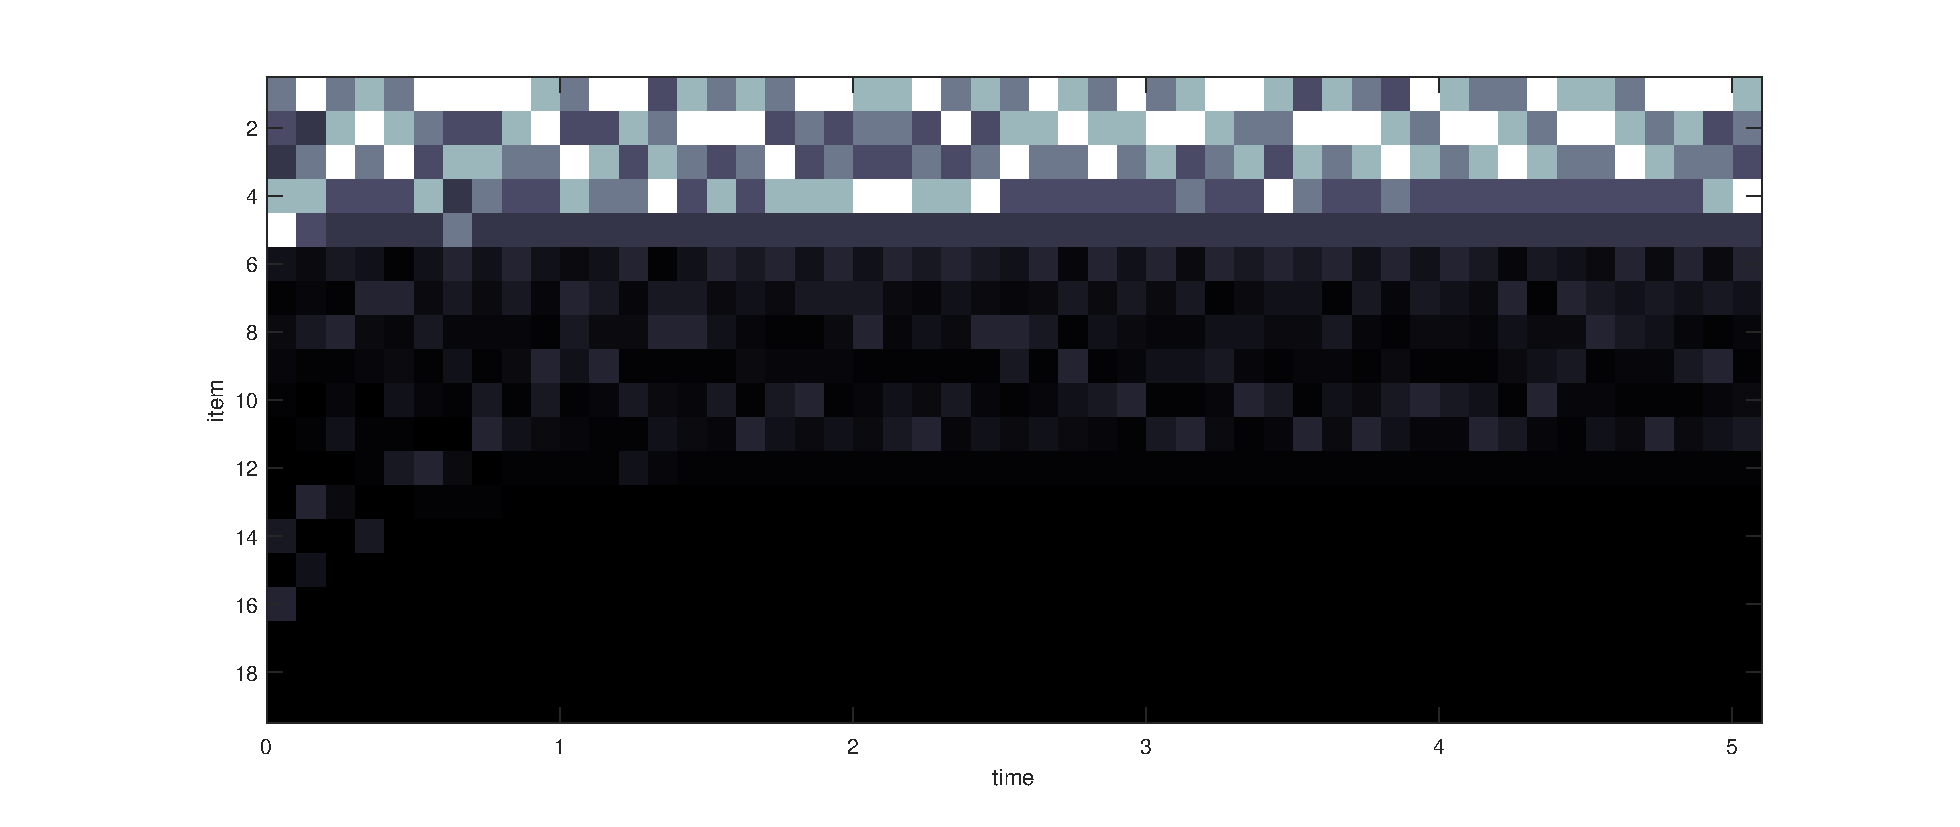
\includegraphics[width = \linewidth]{../model/douhu/pic/hackerNews-heatmap.eps}
		\caption{HackerNews 算法给出的排行榜演化, $x=0.5, \alpha=1.5$}\label{fig:hackerNews-heatmap}
	\end{figure}
	
	\begin{figure}[h!]
		\centering
		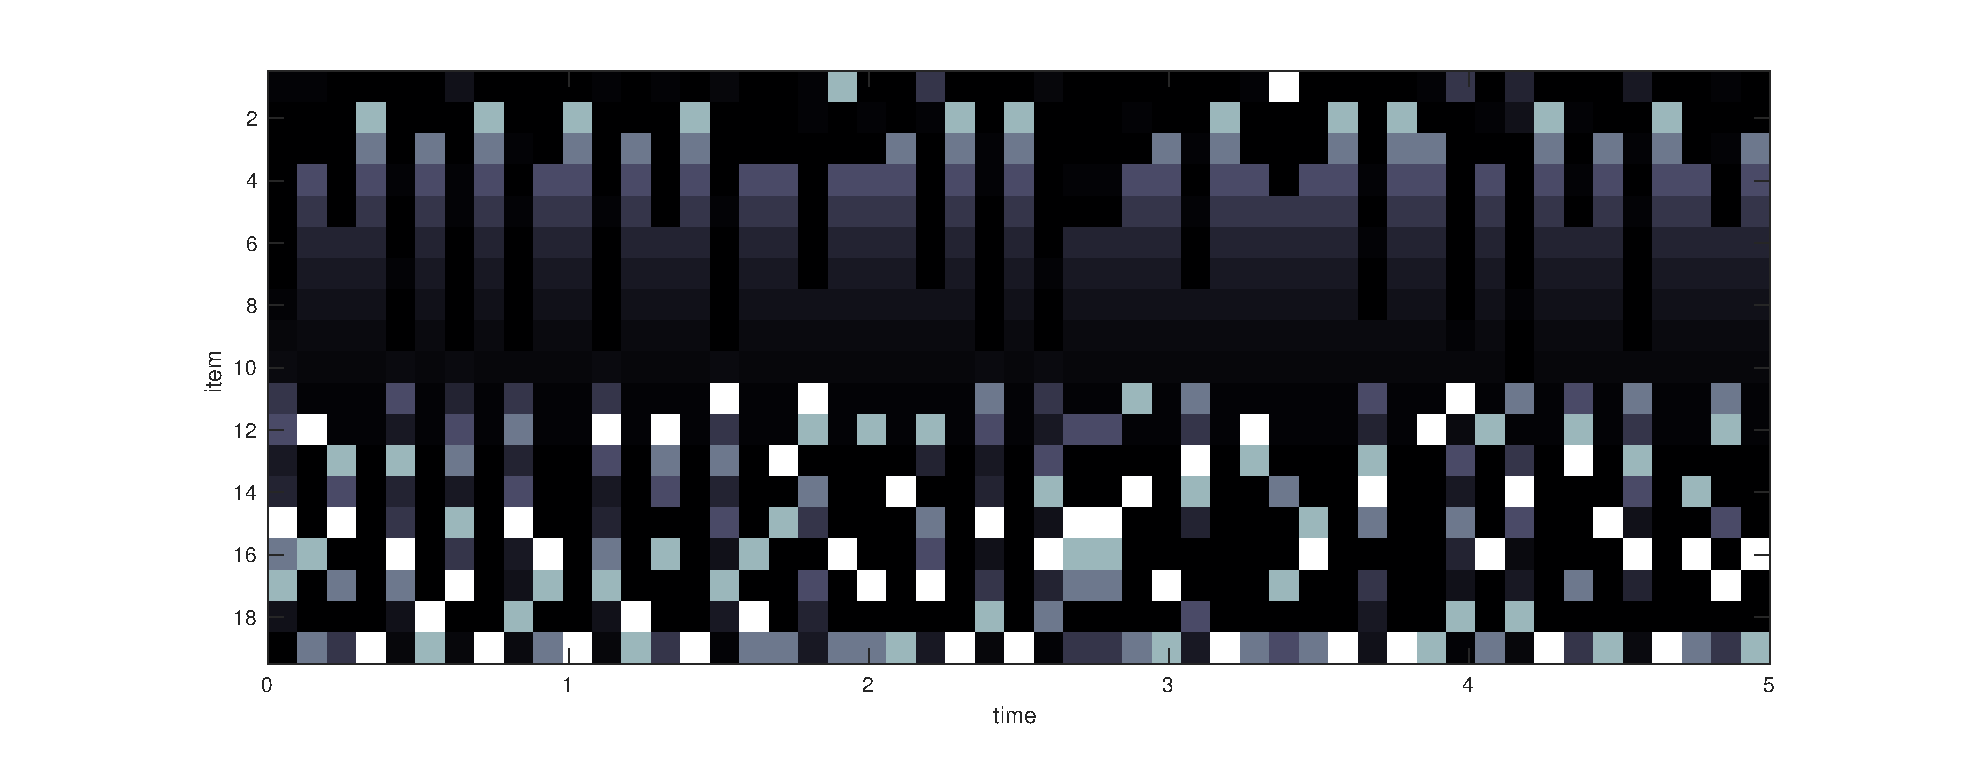
\includegraphics[width = \linewidth]{../model/douhu/pic/ours-heatmap.eps}
		\caption{本文给出的算法给出的排行榜演化, $x=0.5, \alpha=1.5$}\label{fig:ours-heatmap}
	\end{figure}
	可见 Reddit 的热度推荐跳跃太频繁,而 HackerNews 的推荐局限在一个非常小的范围内,受到时间影响很大。本文给出的算法能够很好地均衡以上两种因素。
	
	接下来我们需要观察基于本文算法进行更新的排行榜是否能带给用户更大的快乐。
	\begin{figure}[h!]
		\centering
		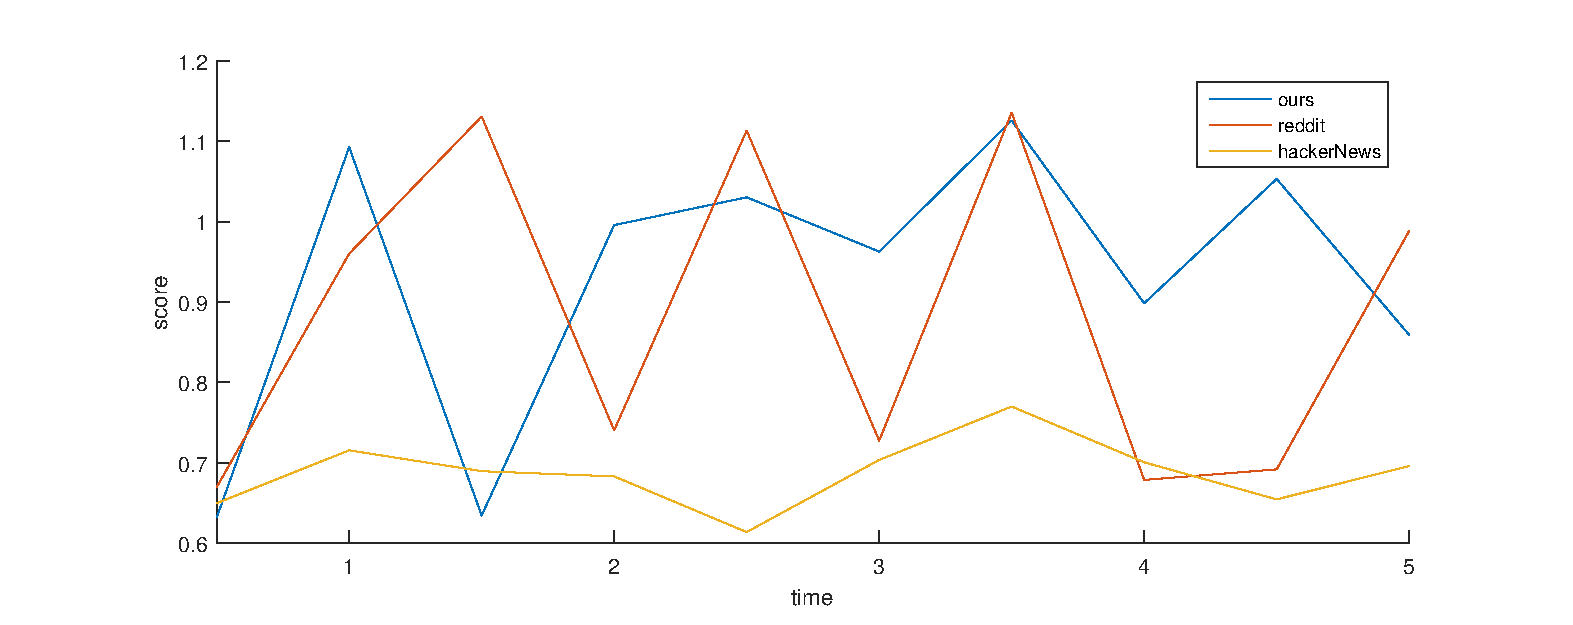
\includegraphics[width = \linewidth]{../model/douhu/pic/three-method-score.eps}
		\caption{三种算法的相应得分变化, $x=0.5, \alpha=1.5$}\label{fig:three-method-score}
	\end{figure}
	可见我们的算法能够比 HackerNews 算法更好,略比 Reddit 算法有优势。如果我们继续观察用户平均浏览时间(见图 \ref{fig:three-method-average-time}):
	\begin{figure}[h!]
		\centering
		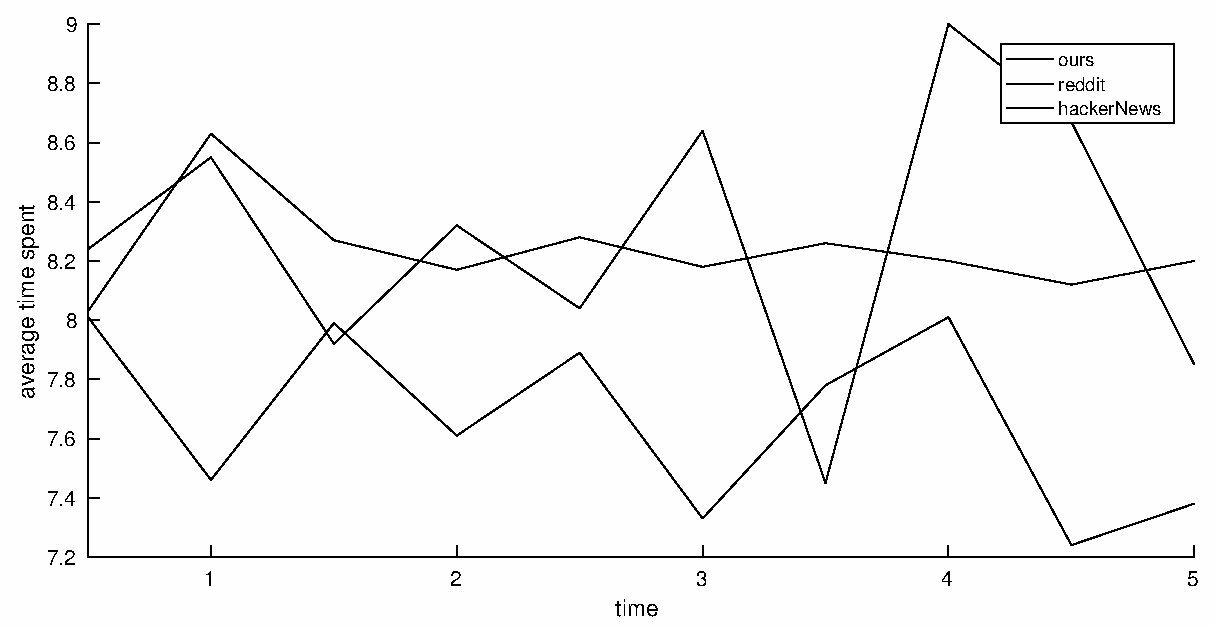
\includegraphics[width = \linewidth]{../model/douhu/pic/three-method-average-time.eps}
		\caption{三种算法的平均浏览时间, $x=0.5, \alpha=1.5$}\label{fig:three-method-average-time}
	\end{figure}
	可知用户平均浏览时间缩短了,但是有效时间并不比另外两种算法要少,说明我们的推荐算法能够令用户在更短时间内看到同样多有趣的内容。

	\section{总结}
	
	\bibliographystyle{plain}
	\bibliography{bib}
	
	\newpage
	\appendix
	\section{定理的证明}
	\begin{thm}\textbf{(无跳过的顺序选择模型)}无跳过顺序选择模型的方差和期望分别为方程(\ref{EQ_A})中所示。
		\begin{equation*}
		\begin{aligned}
		\mathbb{E} \tau_E & = \sum_{k=1}^N \frac{\prod\limits_{j=0}^{k-1}(1-a_{p_j})}{\lambda_{p_i}} \\
		\mathrm{Var} \tau_E & = \sum_{k=1}^N \left(\frac{\prod\limits_{j=0}^{k-1}(1-a_{p_j})}{\lambda_{p_i}}\right)^2
		\end{aligned}
		\end{equation*}
	\begin{proof}[证明]
		取独立指数分布随机变量$\xi_i \sim \mathrm{Exp}(\lambda_i), i = 1, \cdots, N$,则由此跳过程的意义易知
		$$
		\tau_E = \xi_1 + (1-a_{p_1})(\xi_2 + (1-a_{p_2})(\xi_3+\cdots)) = \sum_{k=1}^N \prod_{j=0}^{k-1} (1-a_{p_j}) \xi_k
		$$
		由独立性和指数分布的性质立即得到上面的结果。
	\end{proof}
	\end{thm}
	\begin{thm}\textbf{(带跳过的顺序选择模型)}带跳过的顺序选择模型的方差和期望分别为方程(\ref{EQ_B})中所示。
		\begin{equation*}
		\begin{aligned}
		\mathbb{E} \tau_E & = \sum_{k=1}^N \frac{(1-s_{p_j})\prod\limits_{j=0}^{k-1}(1-a_{p_j})}{\lambda_{p_i}} \\
		\mathrm{Var} \tau_E & = \sum_{k=1}^N (1-s_{p_j}^2)\left(\frac{\prod\limits_{j=0}^{k-1}(1-a_{p_j})}{\lambda_{p_i}}\right)^2
		\end{aligned}
		\end{equation*}
		\begin{proof}[证明]
			将选择是否跳过和阅读的过程所花费的总时间看做互相独立的随机变量$\xi_i$,依然有
			$$
			\tau_E = \xi_1 + (1-a_{p_1})(\xi_2 + (1-a_{p_2})(\xi_3+\cdots)) = \sum_{k=1}^N \prod_{j=0}^{k-1} (1-a_{p_j}) \xi_k
			$$
			此时$\xi_i$的表示变为
			$$
			\xi_i = \zeta_i \tilde{\xi}_i
			$$
			其中
			$\zeta_i \sim \mathrm{Bernoulli}(s_i), \tilde{\xi{i}} \sim \mathrm{Exp}(\lambda_i)$且相互独立。容易计算得到上面的结果。
		\end{proof}
	\end{thm}
	\begin{thm}\textbf{(带跳过的投票模型)}带跳过的投票模型的方差和期望分别为方程(\ref{EQ_C})中所示。
		\begin{equation*}
		\begin{aligned}
		\varphi_{p_j} & = s_{p_j} + n_{p_j} - s_{p_j}n_{p_j} \\
		\mathbb{E} \tau_T & = \sum_{k=1}^N \frac{(1-\varphi_{p_j})\prod\limits_{j=0}^{k-1}(1-t_{p_j})}{\lambda_{p_i}} \\
		\mathrm{Var} \tau_T & = \sum_{k=1}^N (1-\varphi_{p_j}^2)\left(\frac{\prod\limits_{j=0}^{k-1}(1-t_{p_j})}{\lambda_{p_i}}\right)^2
		\end{aligned}
		\end{equation*}
		\begin{proof}[证明]
			将选择是否跳过和阅读的过程的总有效时间看做互相独立的随机变量$\xi_i$,有
			$$
			\tau_E = \xi_1 + (1-t_{p_1})(\xi_2 + (1-t_{p_2})(\xi_3+\cdots)) = \sum_{k=1}^N \prod_{j=0}^{k-1} (1-t_{p_j}) \xi_k
			$$
			此时$\xi_i$的表示变为
			$$
			\xi_i = \zeta_i \eta_i \tilde{\xi}_i
			$$
			其中
			$\zeta_i \sim \mathrm{Bernoulli}(s_i), \eta_i \sim \mathrm{Bernoulli}(n_i), \tilde{\xi{i}} \sim \mathrm{Exp}(\lambda_i)$且相互独立。容易计算得到上面的结果。
		\end{proof}
	\end{thm}
\end{document}
		
		 